%\documentclass{beamer}
\documentclass[handout]{beamer}
\usetheme{Marburg}
\useoutertheme{infolines}
\newcommand{\answers}{1}

\usepackage{amsmath}
\usepackage{caption}
\usepackage{color}
\usepackage{enumerate}
\usepackage{listings}
\usepackage{hyperref}
\usepackage{mathrsfs}
\usepackage{natbib}
\usepackage{url}

\providecommand{\all}{\ \forall \ }
\providecommand{\bs}{\backslash}
\providecommand{\e}{\varepsilon}
\providecommand{\E}{\ \exists \ }
\providecommand{\lm}[2]{\lim_{#1 \rightarrow #2}}
\providecommand{\m}[1]{\mathbb{#1}}
\providecommand{\nv}{{}^{-1}}
\providecommand{\ov}[1]{\overline{#1}}
\providecommand{\p}{\newpage}
\providecommand{\q}{$\quad$ \newline}
\providecommand{\rt}{\rightarrow}
\providecommand{\Rt}{\Rightarrow}
\providecommand{\vc}[1]{\boldsymbol{#1}}
\providecommand{\wh}[1]{\widehat{#1}}

\hypersetup{colorlinks,linkcolor=,urlcolor=blue}
\numberwithin{equation}{section}

\definecolor{dkgreen}{rgb}{0,0.6,0}
\definecolor{gray}{rgb}{0.5,0.5,0.5}
\definecolor{mauve}{rgb}{0.58,0,0.82}

\lstset{ 
  language=C,                % the language of the code
  basicstyle= \footnotesize,           % the size of the fonts that are used for the code
  numberstyle= \tiny \color{white},  % the style that is used for the line-numbers
  stepnumber=2,                   % the step between two line-numbers. 
  numbersep=5pt,                  % how far the line-numbers are from the code
  backgroundcolor=\color{white},      % choose the background color. You must add \usepackage{color}
  showspaces=false,               % show spaces adding particular underscores
  showstringspaces=false,         % underline spaces within strings
  showtabs=false,                 % show tabs within strings adding particular underscores
  frame=lrb,                   % adds a frame around the code
  rulecolor=\color{black},        % if not set, the frame-color may be changed on line-breaks within not-black text 
  tabsize=2,                      % sets default tabsize to 2 spaces
  captionpos=t,                   % sets the caption-position 
  breaklines=true,                % sets automatic line breaking
  breakatwhitespace=false,        % sets if automatic breaks should only happen at whitespace
  %title=\lstname,                   % show the filename of files included with \lstinputlisting;
  keywordstyle=\color{blue},          % keyword style
  commentstyle=\color{gray},       % comment style
  stringstyle=\color{dkgreen},         % string literal style
  escapeinside={\%*}{*)},            % if you want to add LaTeX within your code
  morekeywords={*, ...},               % if you want to add more keywords to the set
  xleftmargin=0.053in, % left horizontal offset of caption box
  xrightmargin=-.03in % right horizontal offset of caption box
}

%\DeclareCaptionFont{white}{\color{white}}
%\DeclareCaptionFormat{listing}{\parbox{\textwidth}{\colorbox{gray}{\parbox{\textwidth}{#1#2#3}}\vskip-0.05in}}
%\captionsetup[lstlisting]{format = listing, labelfont = white, textfont = white}
%For caption-free listings, comment out the 3 lines above and uncomment the 2 lines below.
 \captionsetup{labelformat = empty, labelsep = none}
 \lstset{frame = single}

\title{A codelsss introduction to GPU parallelism}
\author{Will Landau}
\date{September 23, 2013}
\institute{Iowa State University}

\begin{document}
 
 
 \begin{frame}
\titlepage
 \end{frame}
 
 
\begin{frame}
\frametitle{Outline}
\tableofcontents
\end{frame}
 
 
 \AtBeginSection[]
{
   \begin{frame}
       \frametitle{Outline}
       \tableofcontents[currentsection]
   \end{frame}
}


\section{A review of GPU parallelism}



\begin{frame}[fragile]
\frametitle{The single instruction, multiple data (SIMD) paradigm}

\begin{itemize}
\pause \item SIMD: apply the same command to multiple places in a dataset. 

\pause \begin{lstlisting}
for(i = 0; i < 1e6; ++i)
  a[i] = b[i] + c[i];
\end{lstlisting}


\pause \item On CPUs, the iterations of the loop run sequentially.

\pause \item With GPUs, we can easily run all 1,000,000 iterations simultaneously.

\pause \begin{lstlisting}
i = threadIdx.x;
a[i] = b[i] + c[i];
\end{lstlisting}

\pause \item We can similarly \emph{parallelize} a lot more than just loops.
\end{itemize}
\end{frame}


\begin{frame}
\frametitle{CPU / GPU cooperation}

\begin{itemize}
\item The CPU (``host") is in charge.
\uncover<2->{\item The CPU sends computationally intensive instruction sets to the GPU (``device") just like a human uses a pocket calculator.}
\end{itemize}

\begin{center}
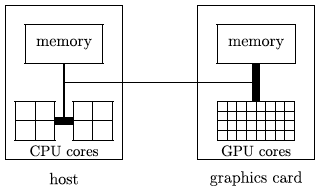
\includegraphics[scale=.8]{../../fig/communication.png}
\end{center}
\end{frame}


\begin{frame}
\frametitle{How GPU parallelism works}
\begin{enumerate}
\item The CPU sends a command called a {\bf kernel} to a GPU.
\pause \item The GPU executes several duplicate realizations of this command, called {\bf threads}.
\begin{itemize}
\pause \item These threads are grouped into bunches called {\bf blocks}.
\pause \item The sum total of all threads in a kernel is called a {\bf grid}.
\end{itemize}
\end{enumerate}

\begin{itemize}
\item Toy example:
\begin{itemize}
\item CPU says: ``Hey, GPU. Sum pairs of adjacent numbers. Use the array, (1, 2, 3, 4, 5, 6, 7, 8)."
\pause \item GPU thinks: ``Sum pairs of adjacent numbers" is a kernel that I need to apply to the array, (1, 2, 3, 4, 5, 6, 8).
\pause \item The GPU spawns 2 blocks, each with 2 threads:
\end{itemize}
\end{itemize}

\pause \begin{center}
\begin{tabular}{c|cc|cc}
Block  & \multicolumn{2}{c|}{0} &  \multicolumn{2}{c}{1} \\ \hline
Thread & 0 & 1 & 0 & 1  \\ \hline
Action & 1 + 2 & 3 + 4 & 5 + 6 & 7 + 8 \\
\end{tabular}
\end{center}

\begin{itemize}
\pause \item I could have also used 1 block with 4 threads and given the threads different pairs of numbers.
\end{itemize}
\end{frame}

\begin{frame}
\begin{center}
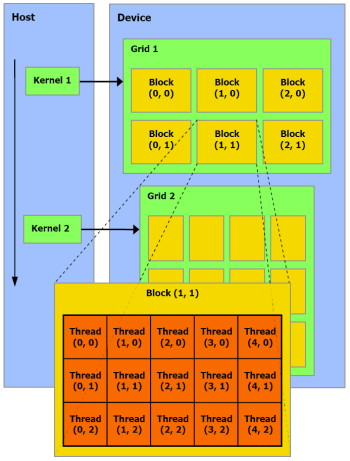
\includegraphics[scale=.7]{../../fig/gridBlocksThreads.jpg}
\end{center}
\end{frame}


\section{Examples of parallelism}


\subsection{Vector addition}

\begin{frame}
\frametitle{Vector addition}


\begin{itemize}
\item Say I have 2 vectors,


\begin{align*}
a = \begin{bmatrix} a_1 \\ a_2 \\ \vdots \\ a_n \end{bmatrix} \qquad b = \begin{bmatrix} b_1 \\ b_2 \\ \vdots \\ b_n  \end{bmatrix}
\end{align*}

\pause \item I want to compute their component-wise sum,
\begin{align*}
c = \begin{bmatrix} c_1 \\ c_2 \\ \vdots \\ c_n \end{bmatrix} = \begin{bmatrix} a_1 + b_1 \\ a_2 + b_2 \\ \vdots \\ a_n + b_n  \end{bmatrix}
\end{align*}

\end{itemize}
\end{frame}

\begin{frame}
\frametitle{Vector addition}
\begin{center}
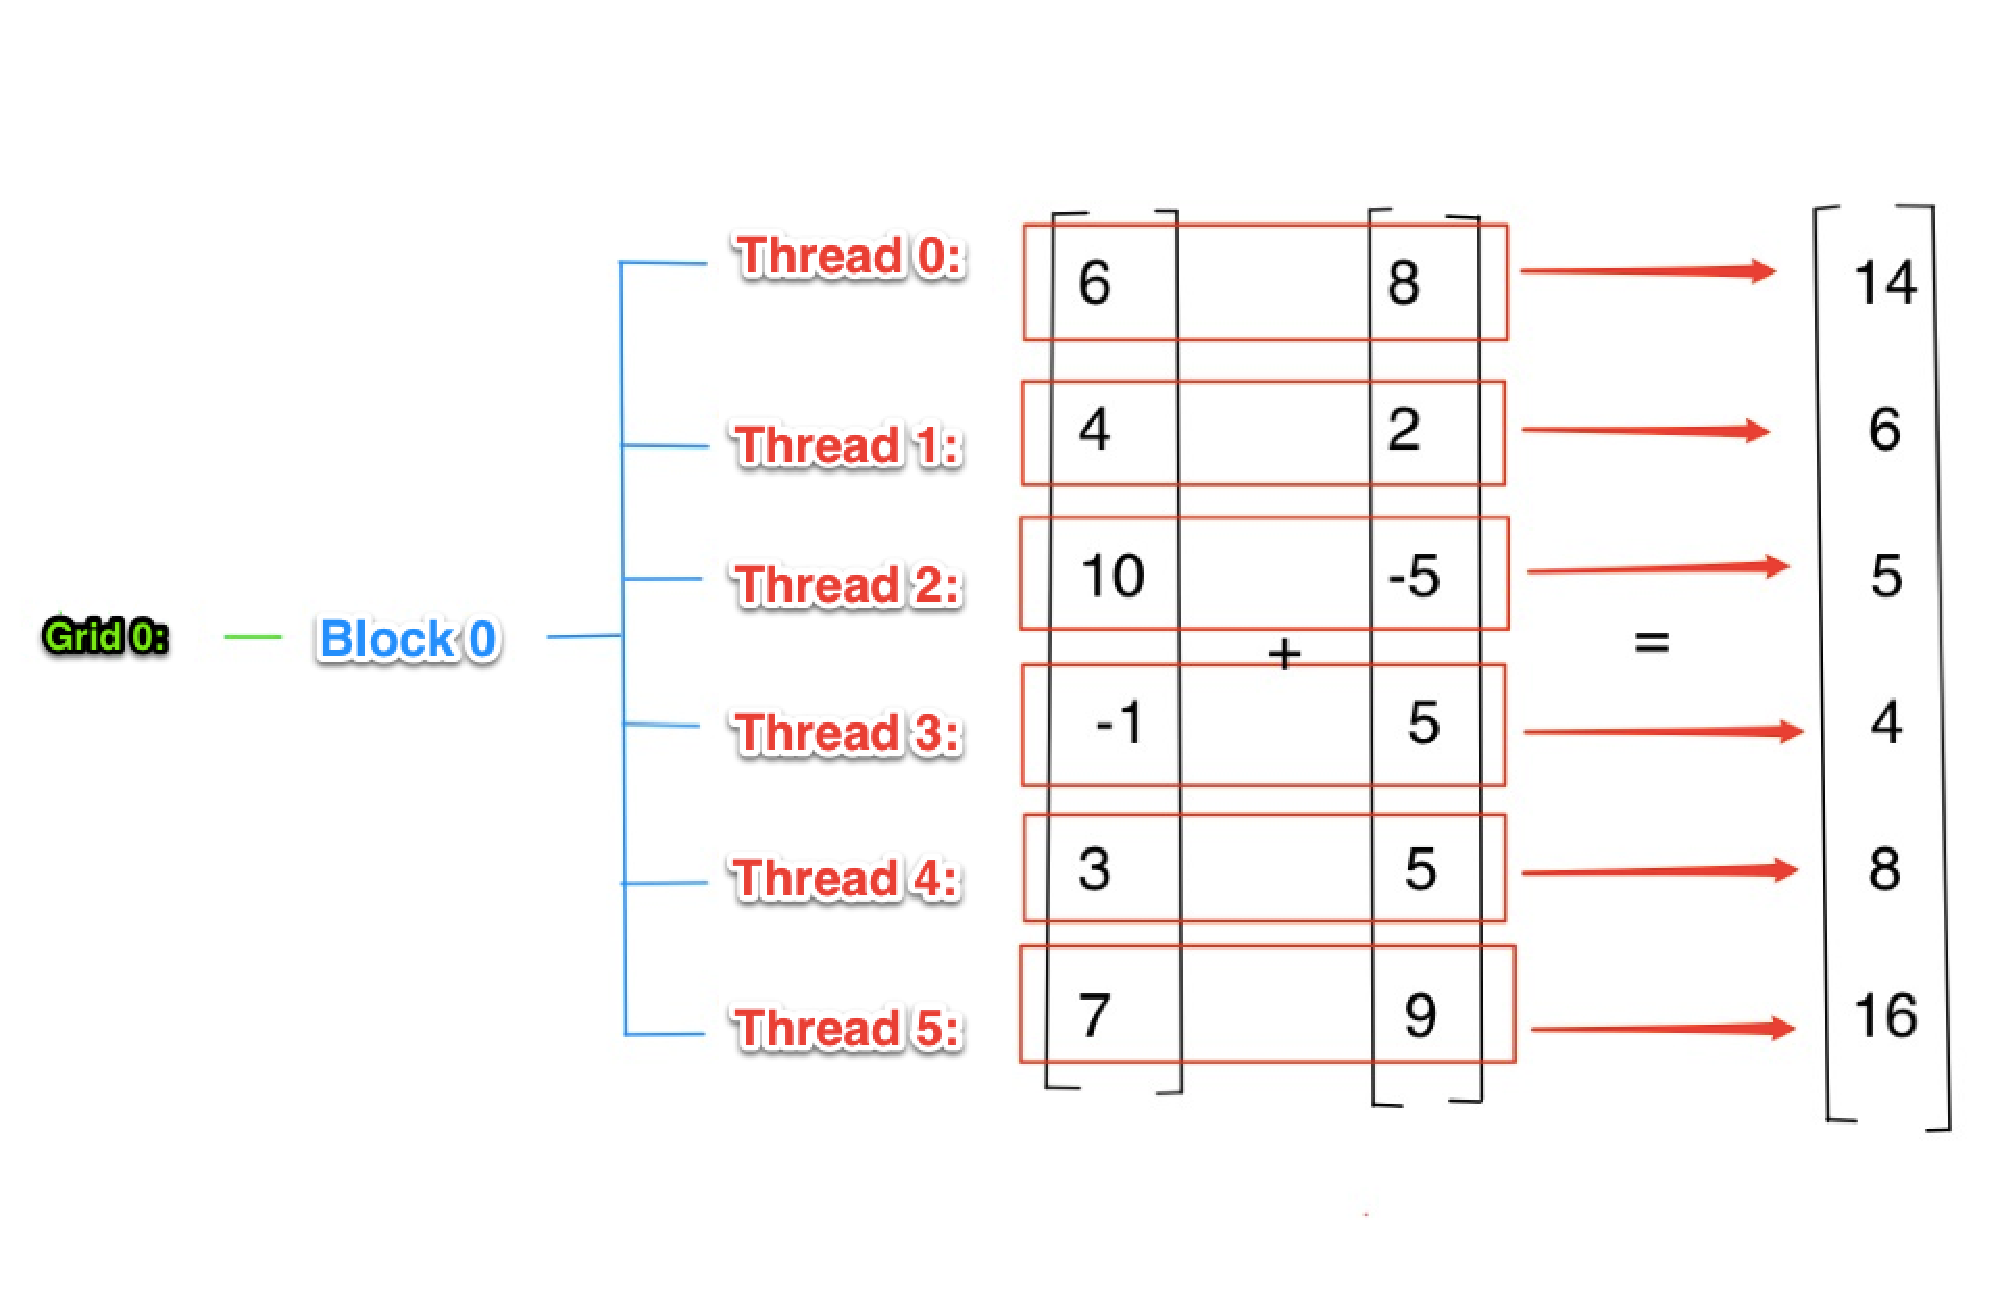
\includegraphics[scale=.25]{../../fig/vadd1.pdf}
\end{center}
\end{frame}


\begin{frame}
\frametitle{Vector addition}
\begin{center}
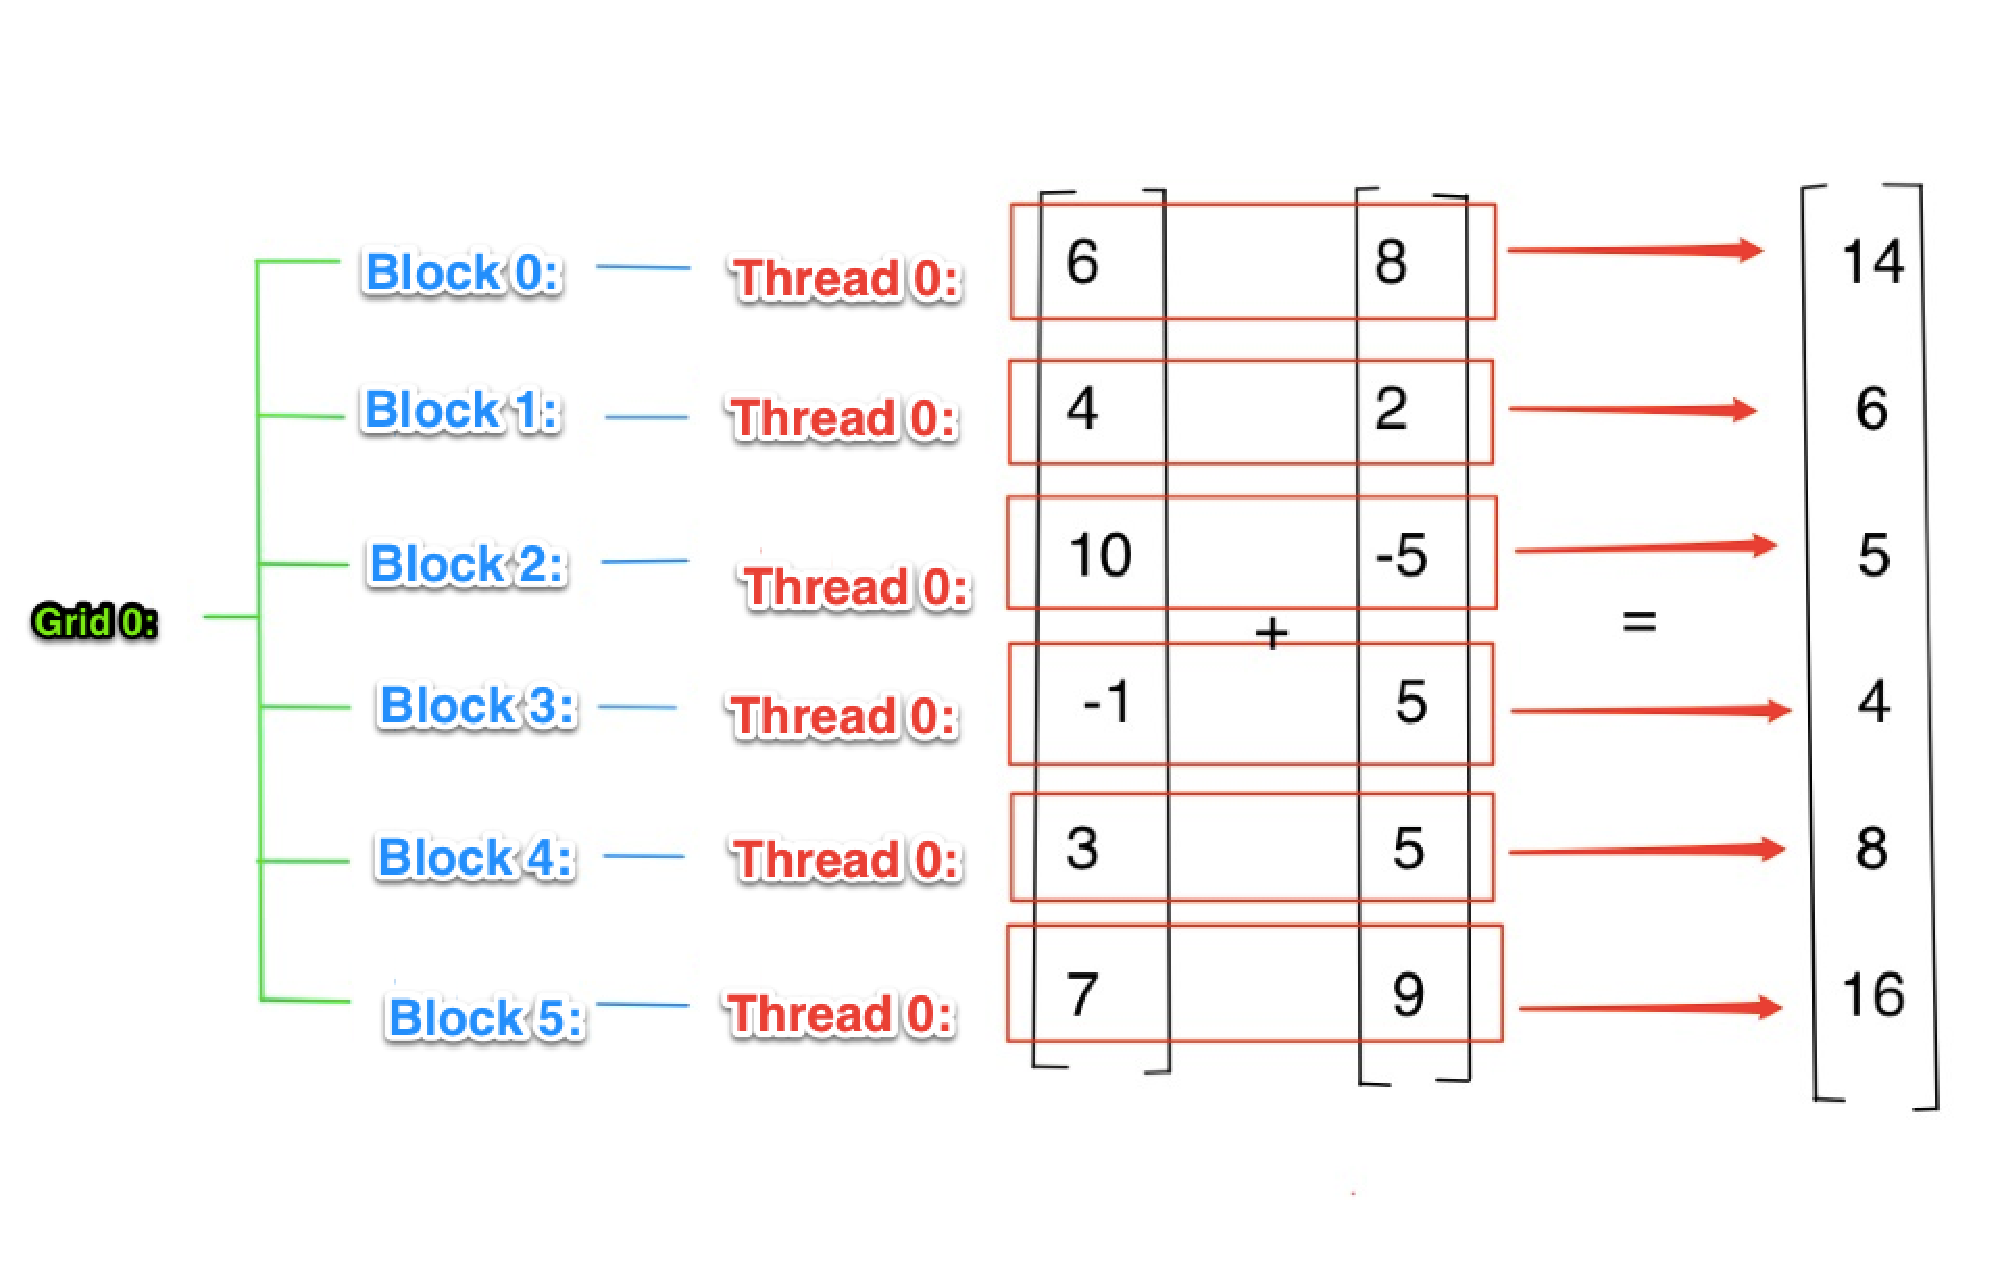
\includegraphics[scale=.25]{../../fig/vadd2.pdf}
\end{center}
\end{frame}

\begin{frame}
\frametitle{Vector addition}
\begin{center}
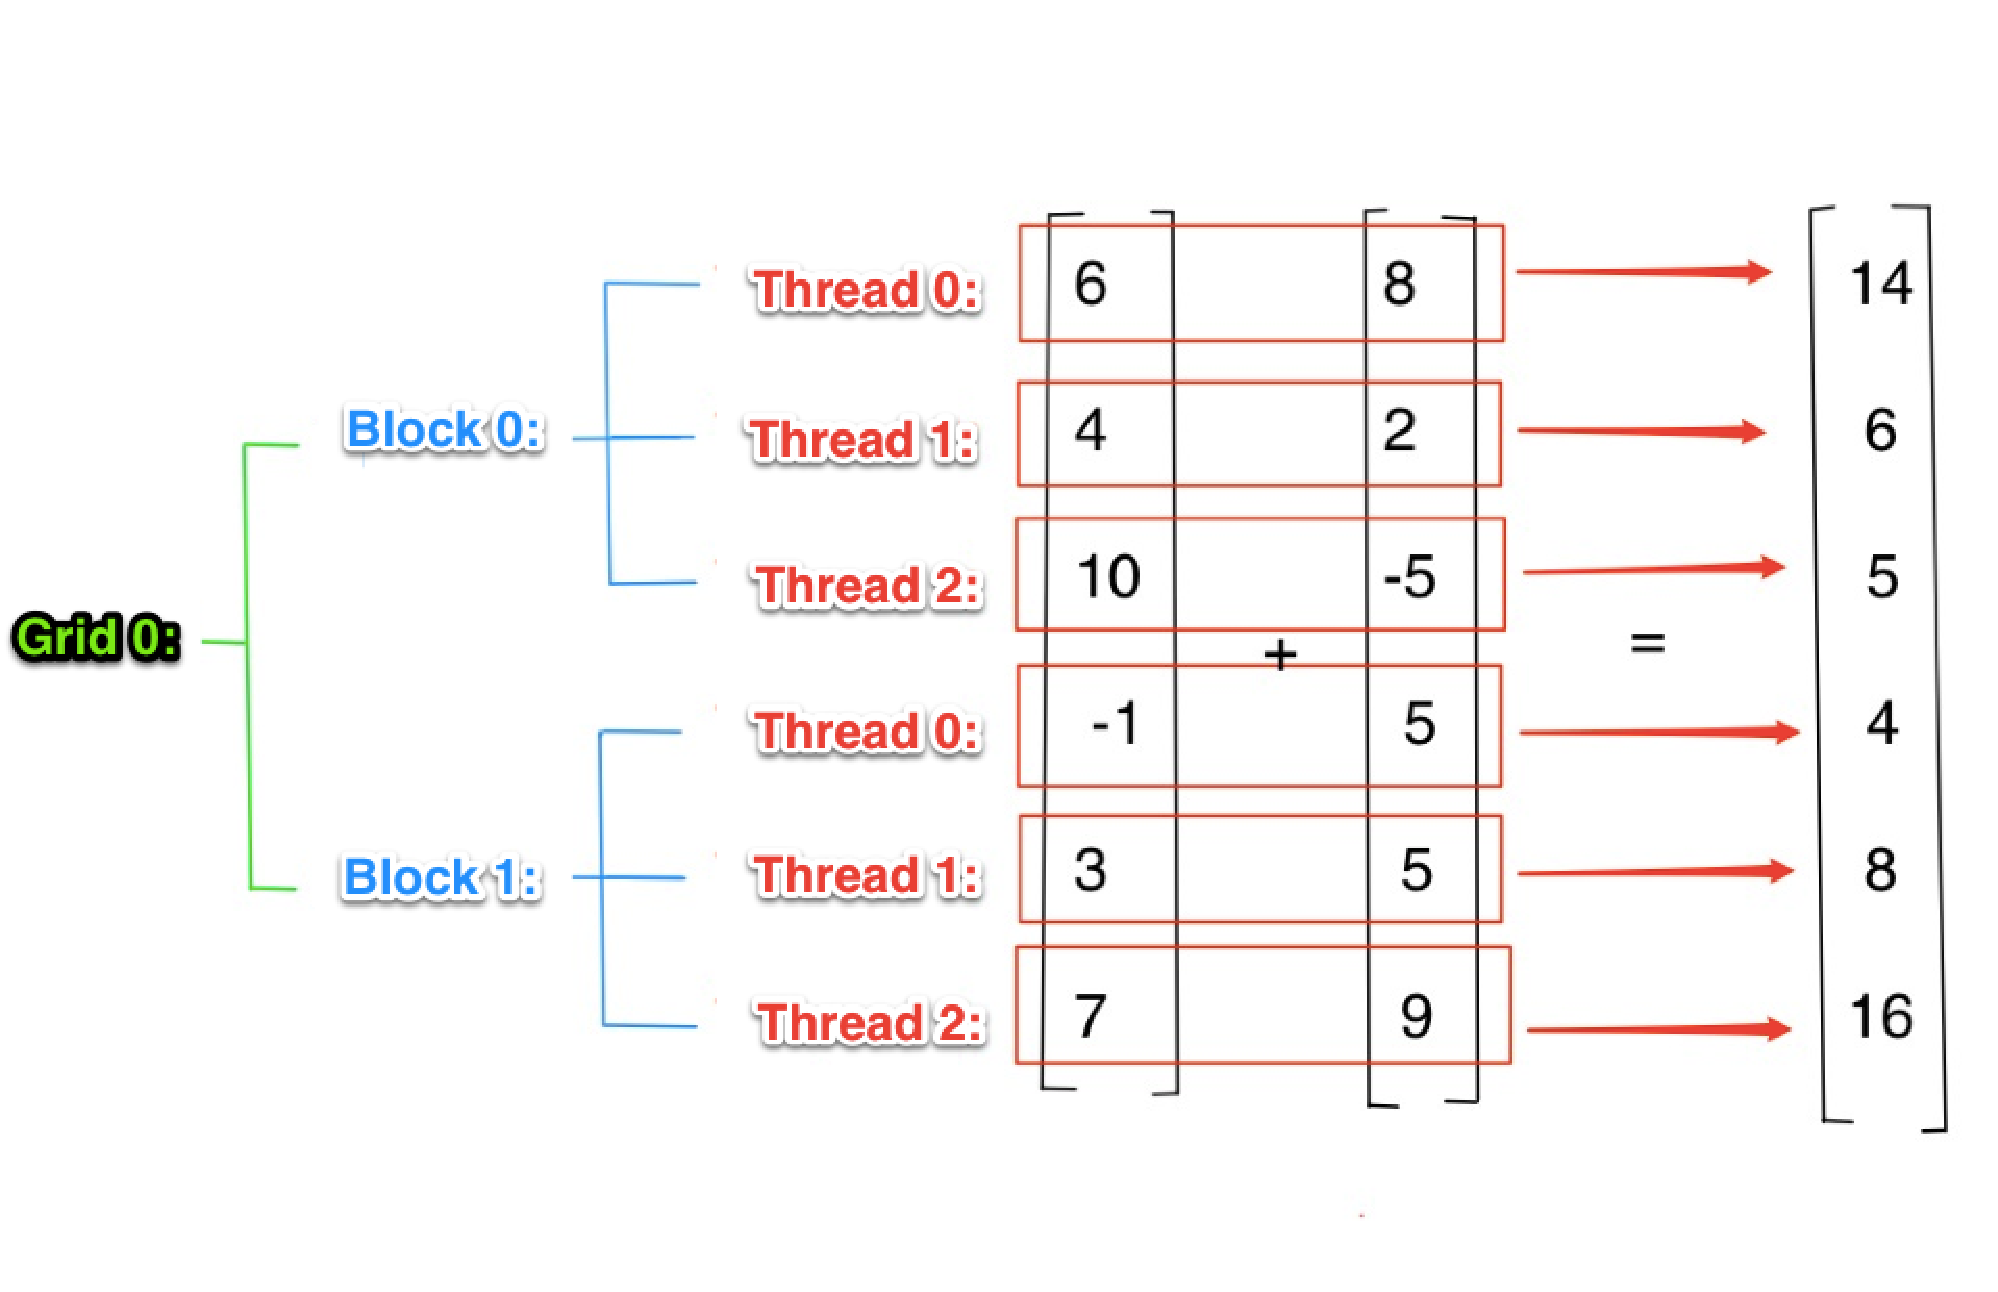
\includegraphics[scale=.25]{../../fig/vadd3.pdf}
\end{center}
\end{frame}

\subsection{Pairwise summation}


\begin{frame}
\frametitle{Pairwise summation}

\begin{itemize}
\item Let's take the pairwise sum of the vector,

\begin{align*}
(5, 2, -3, 1, 1, 8, 2, 6)
\end{align*}

using 1 block of 4 threads.
\end{itemize}
\end{frame}

\begin{frame}
\frametitle{Pairwise summation}
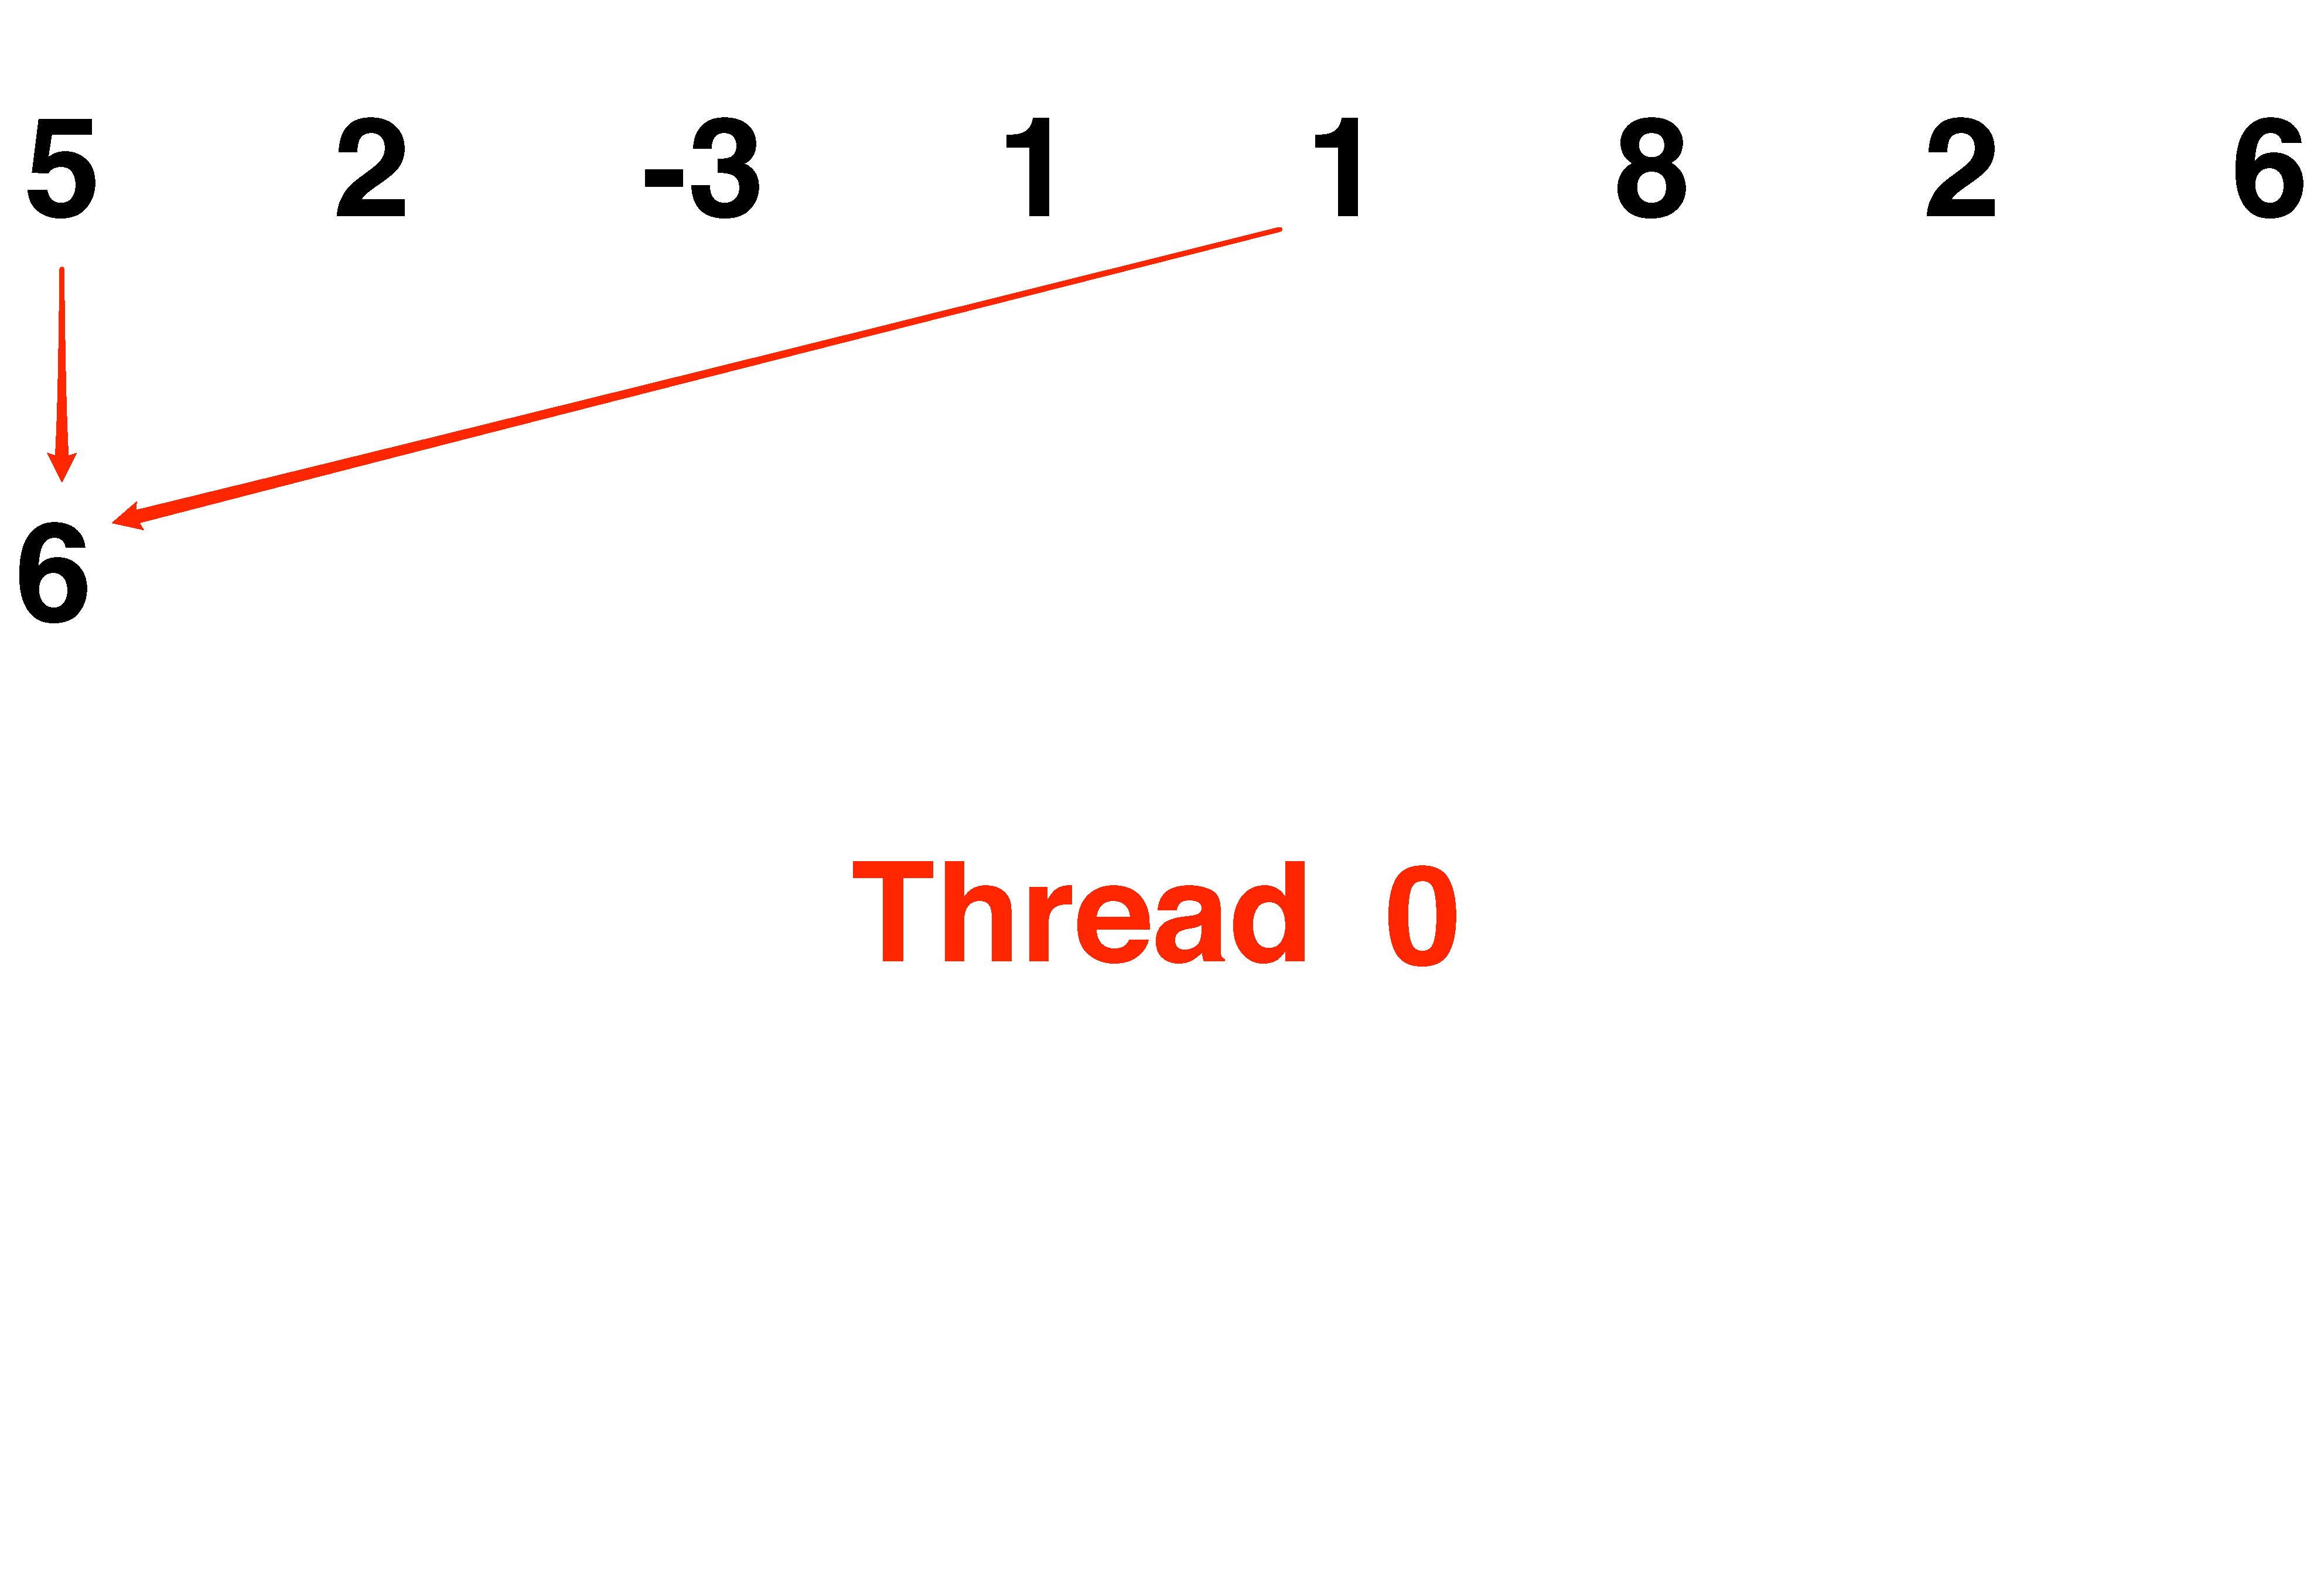
\includegraphics[scale=.15]{../../fig/psum1.pdf}
\end{frame}

\begin{frame}
\frametitle{Pairwise summation}
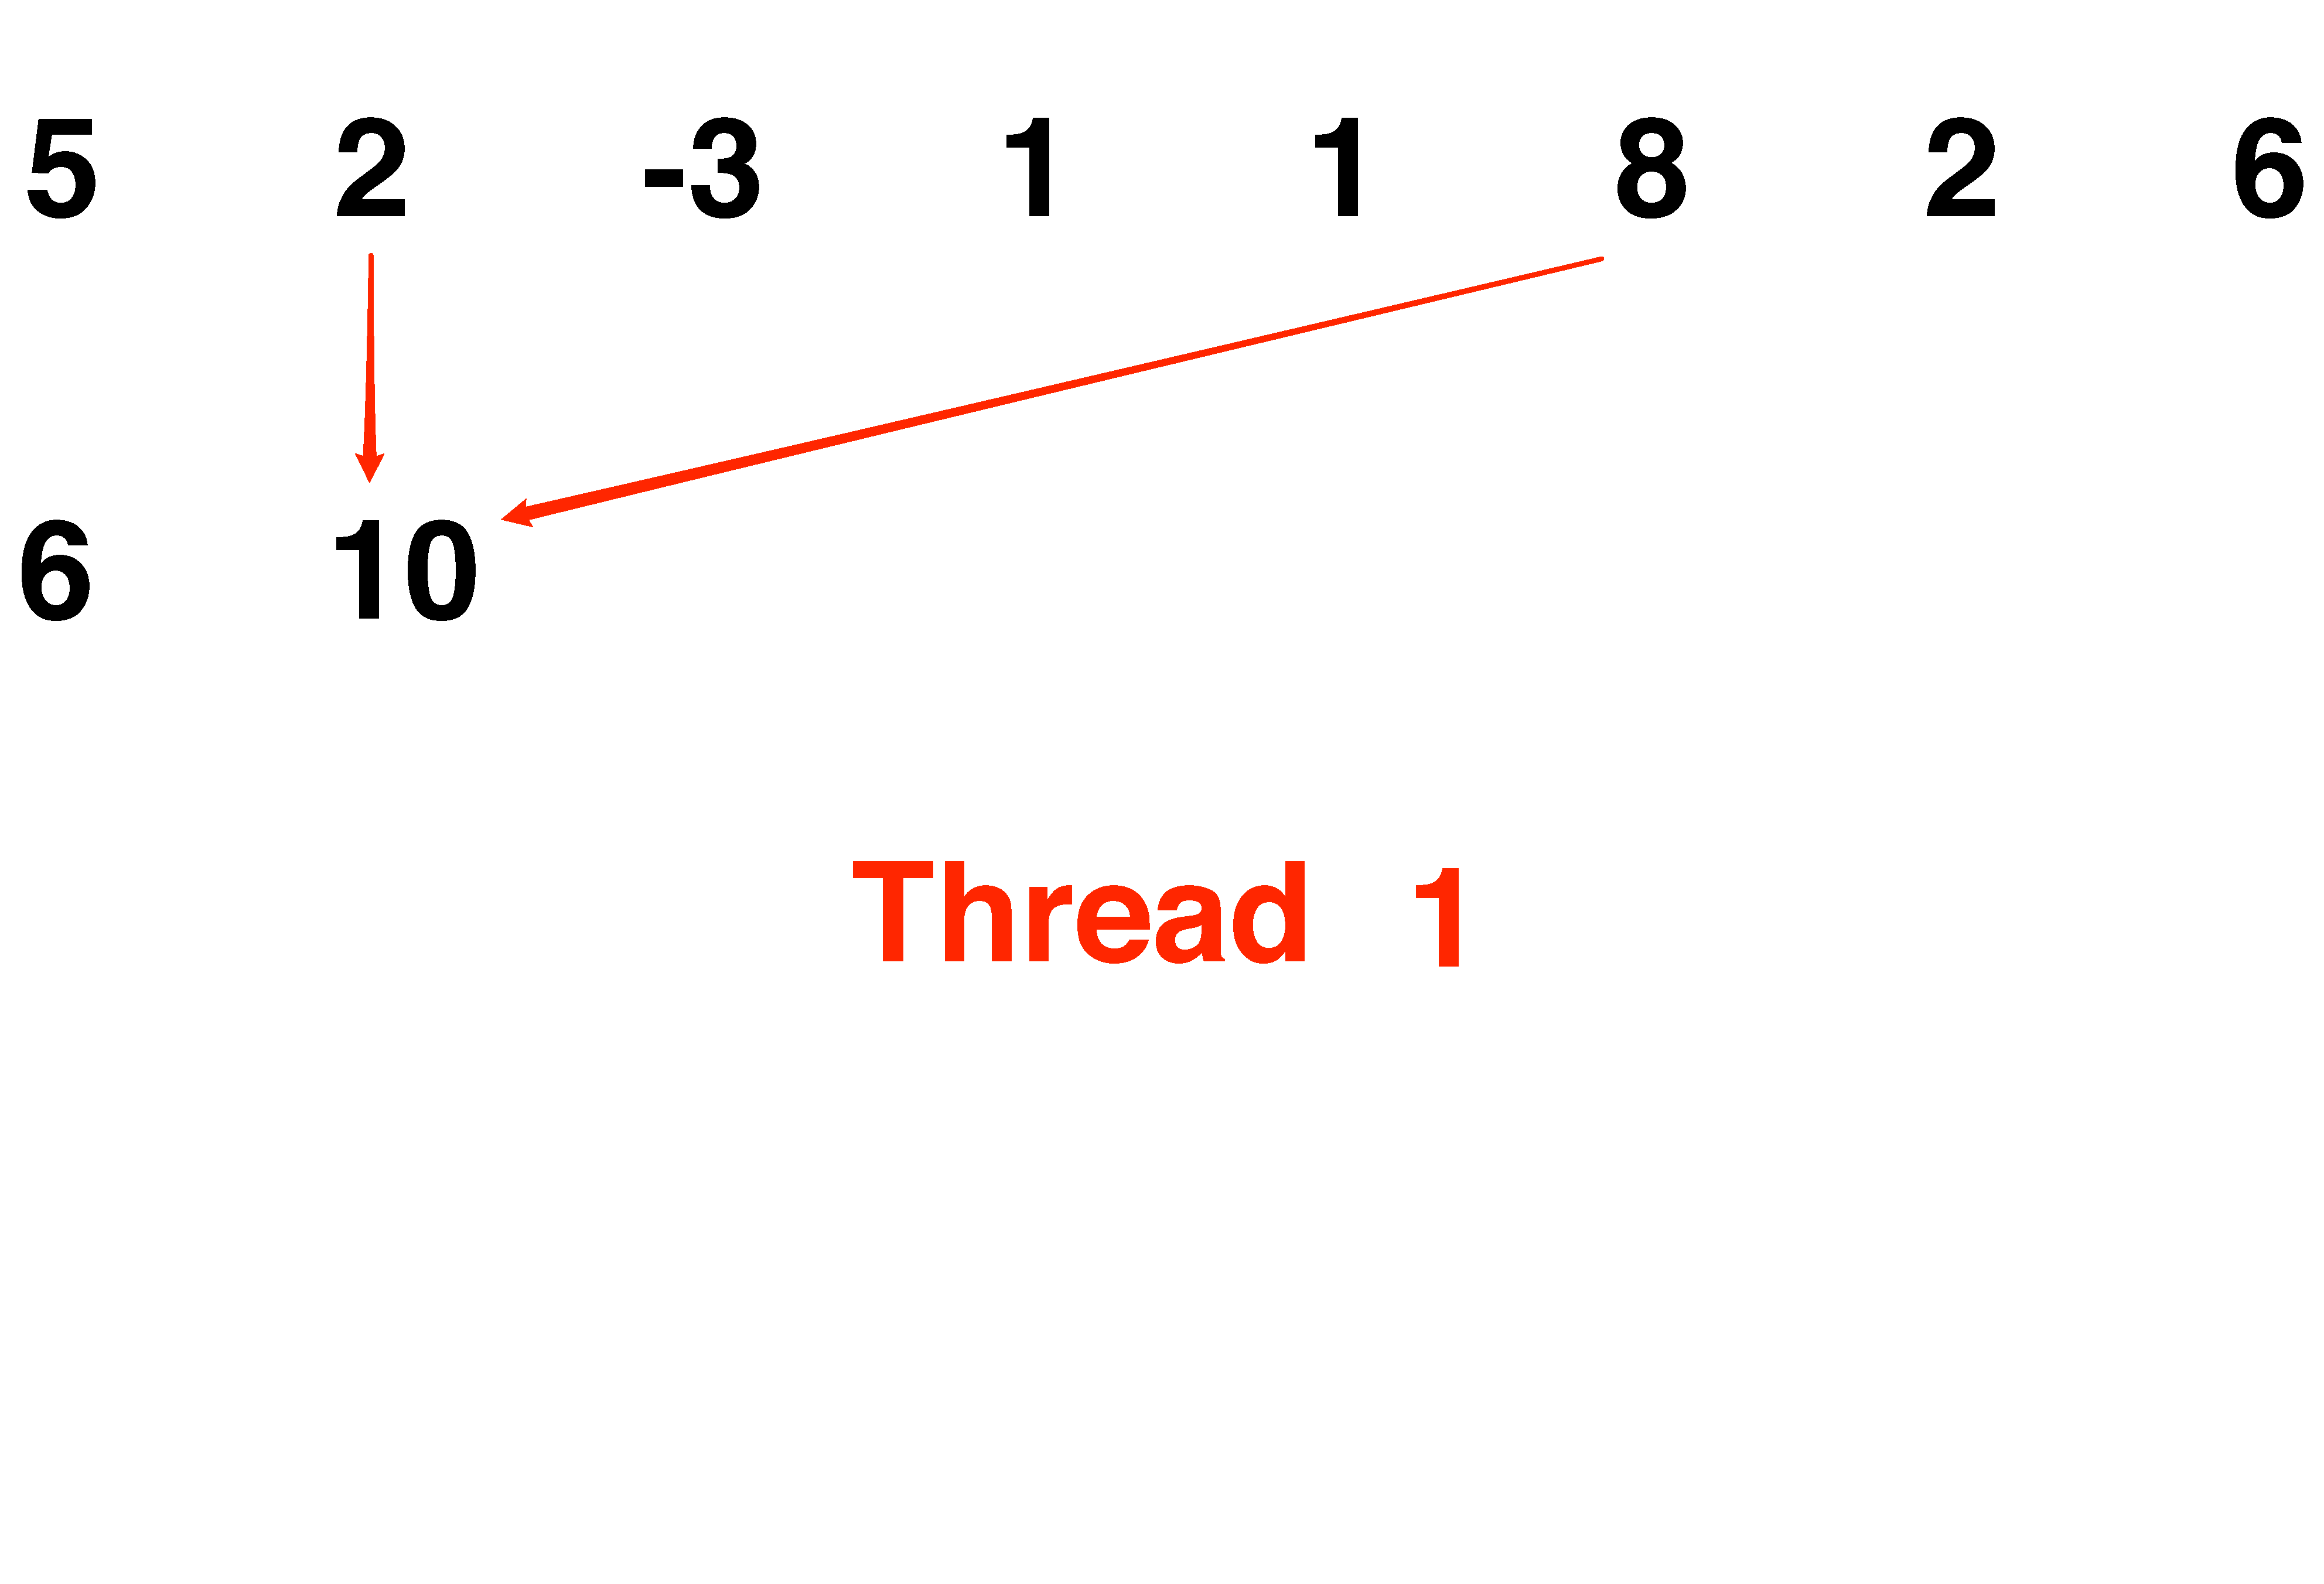
\includegraphics[scale=.15]{../../fig/psum2.pdf}
\end{frame}

\begin{frame}
\frametitle{Pairwise summation}
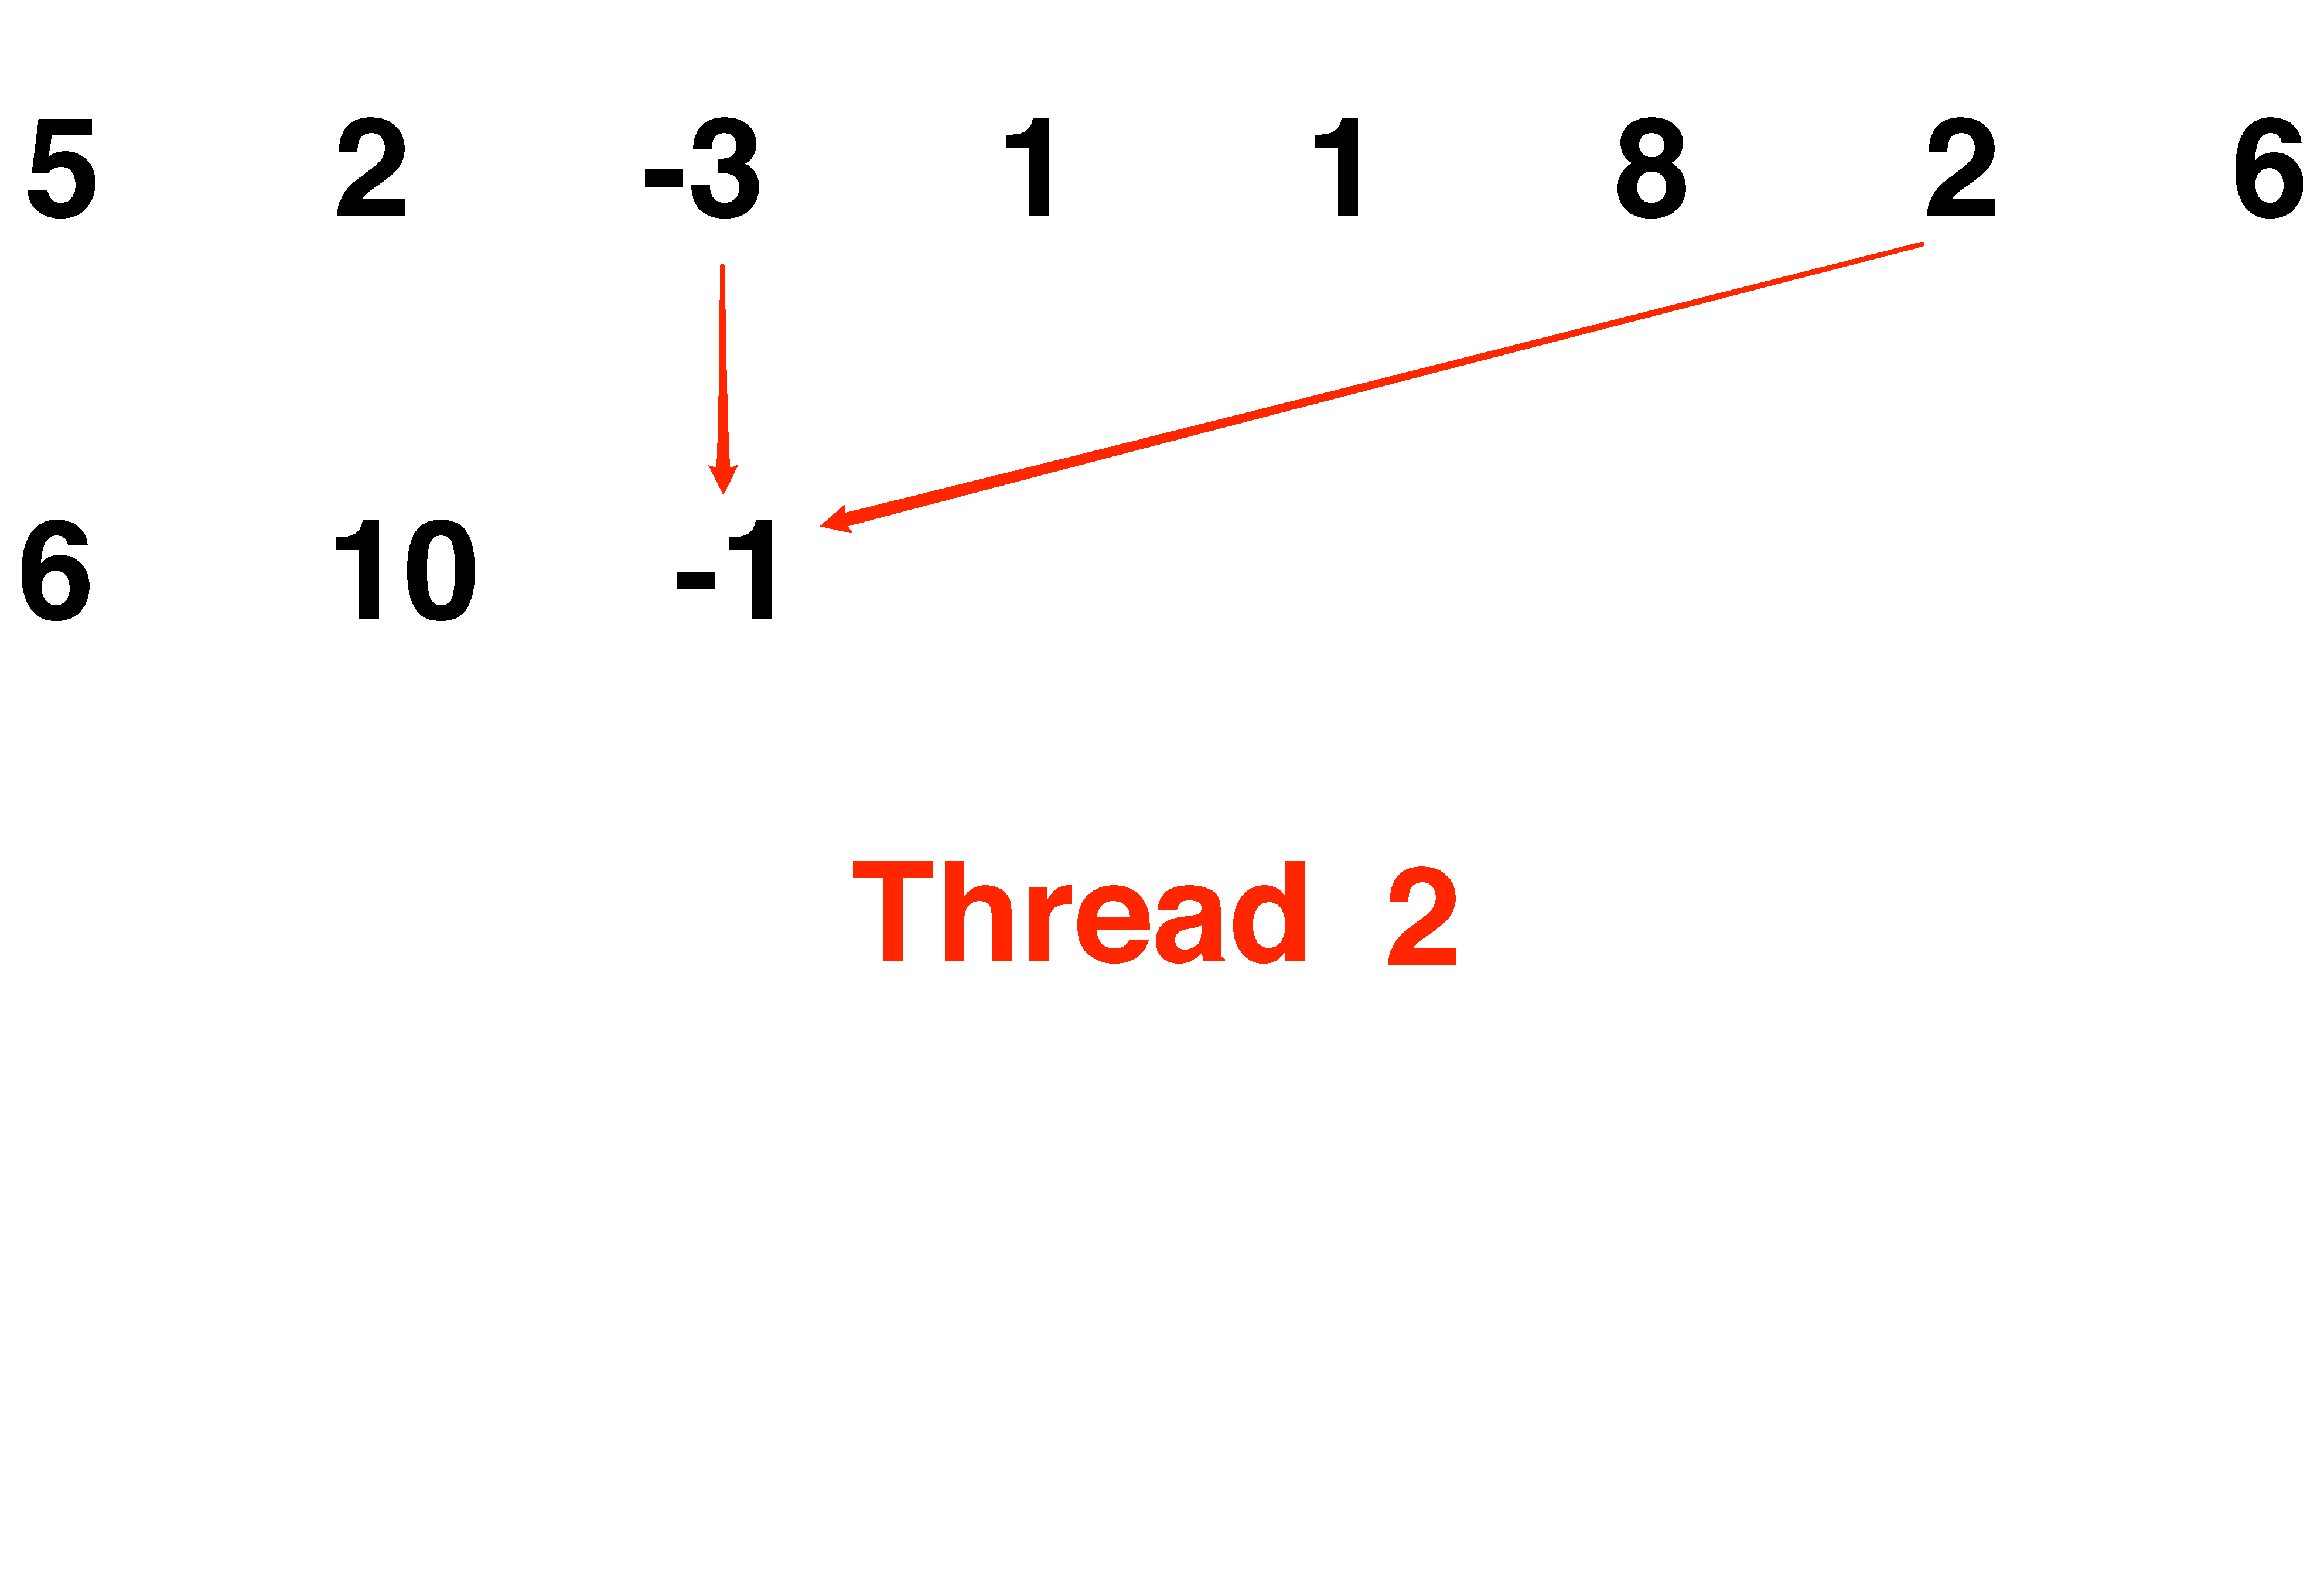
\includegraphics[scale=.15]{../../fig/psum3.pdf}
\end{frame}
{}
\begin{frame}
\frametitle{Pairwise summation}
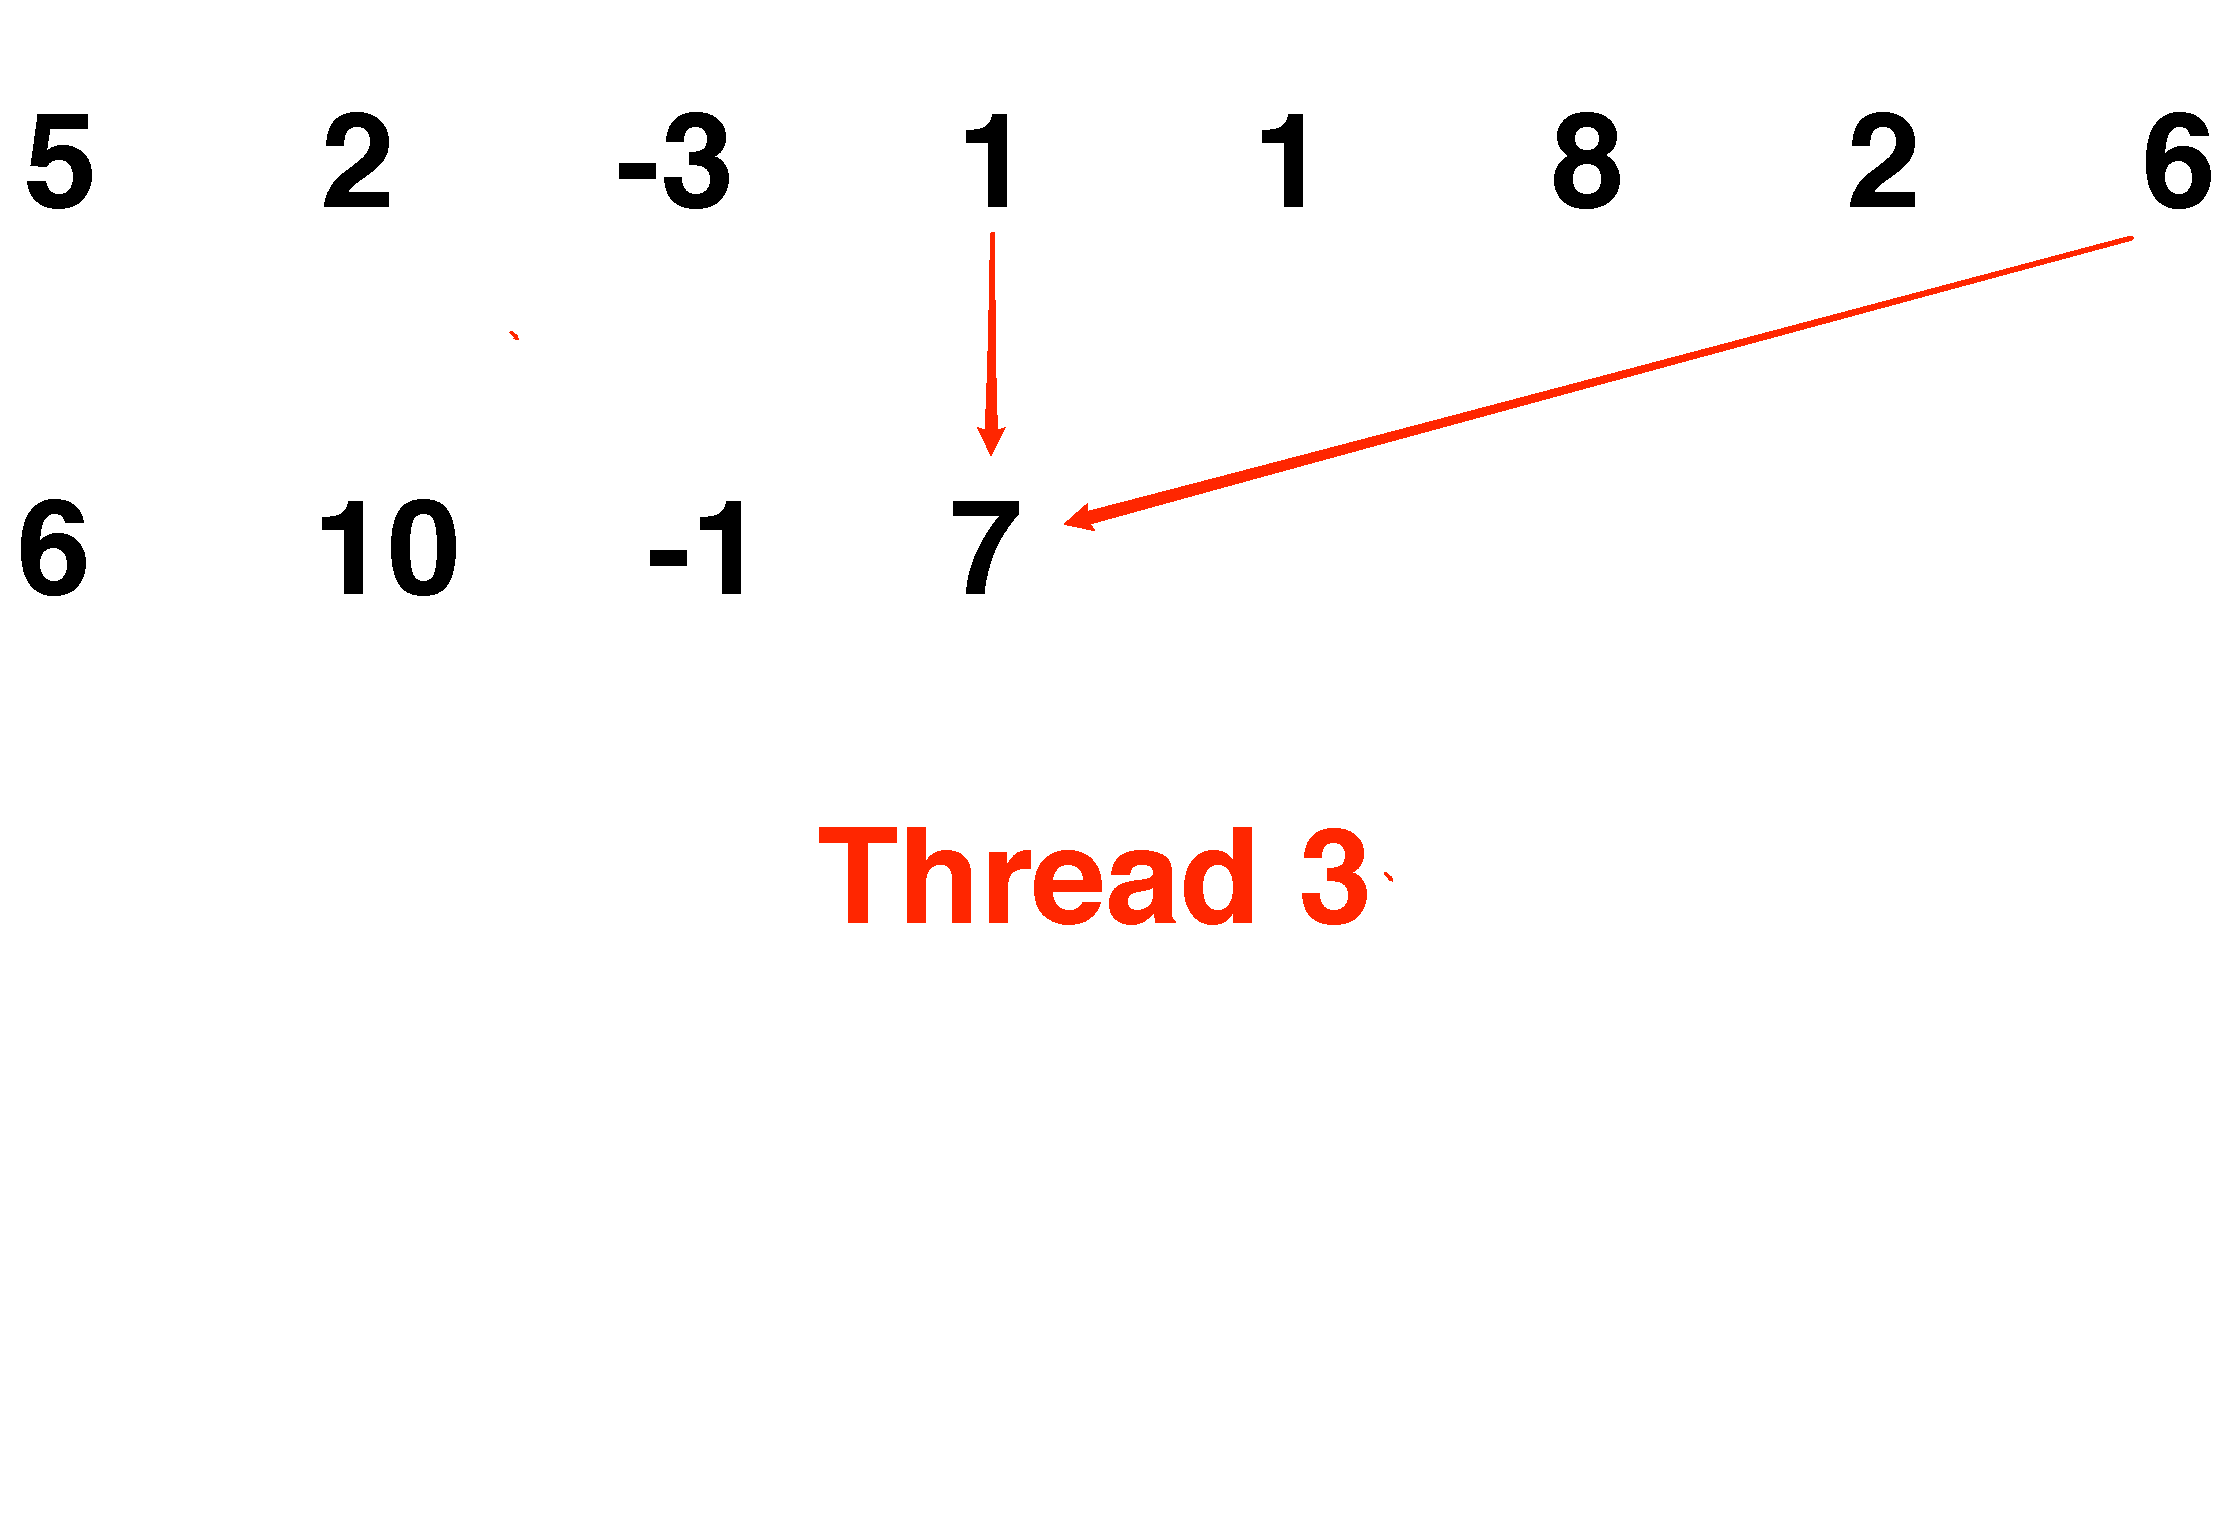
\includegraphics[scale=.25]{../../fig/psum4.pdf}
\end{frame}

\begin{frame}
\frametitle{Pairwise summation}
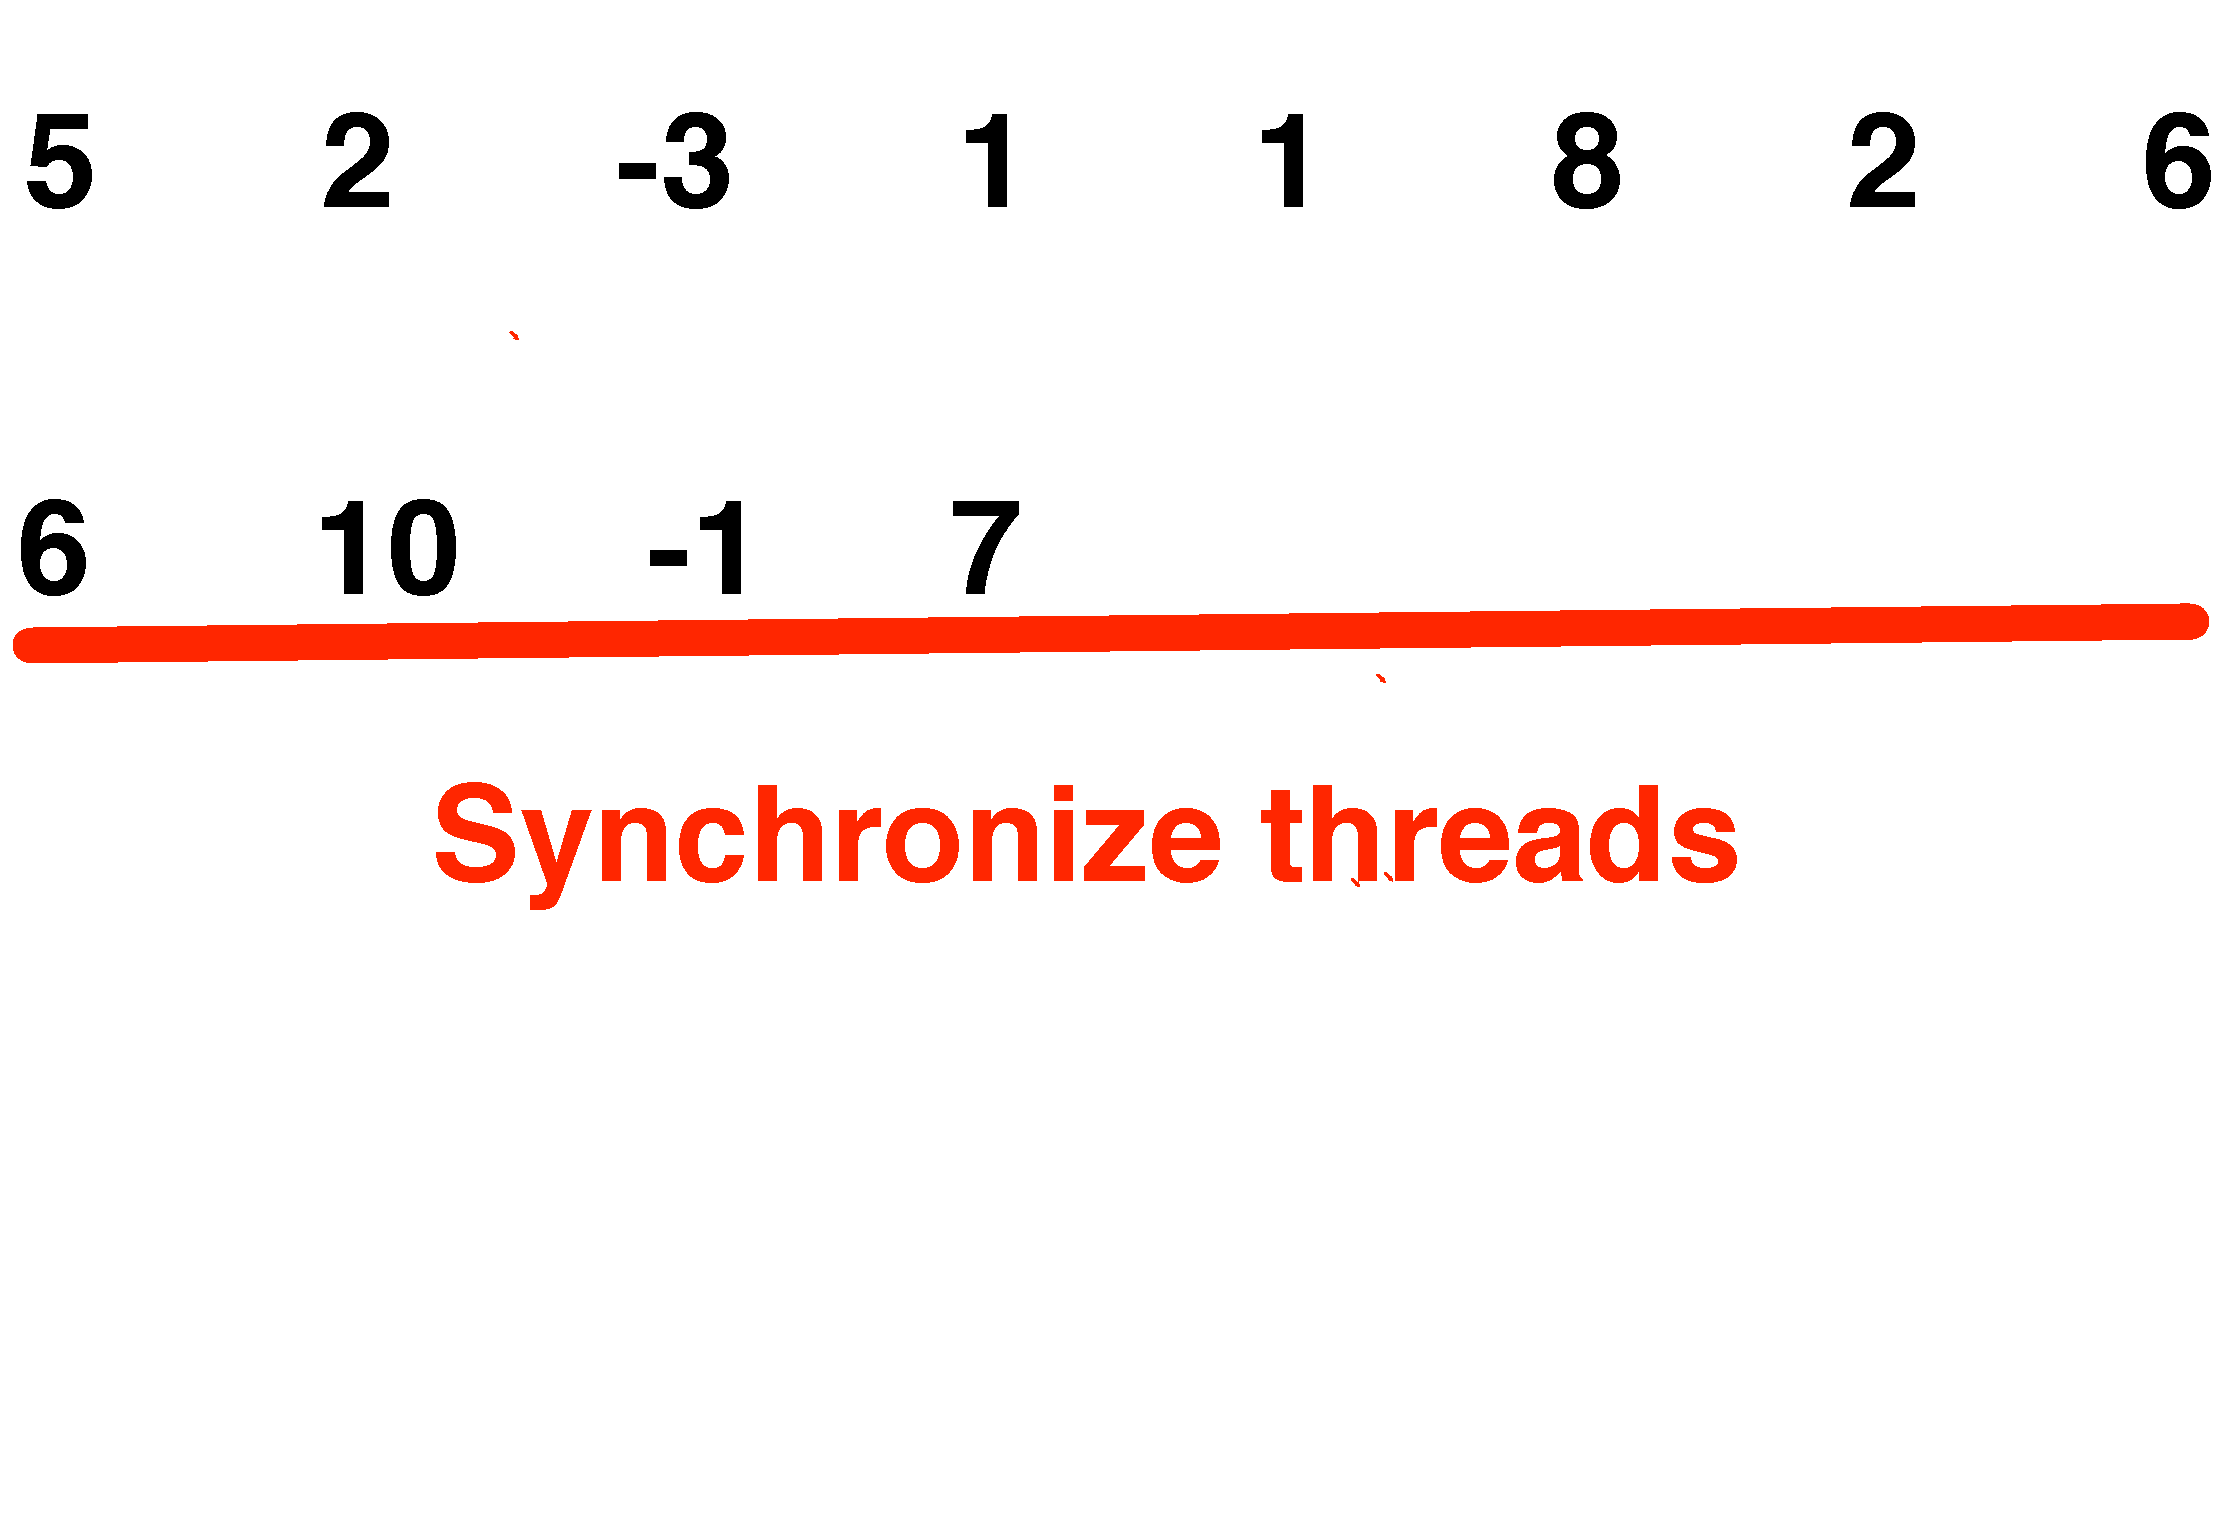
\includegraphics[scale=.25]{../../fig/psum5.pdf}
\end{frame}

\begin{frame}
\frametitle{Synchronizing threads}
\begin{itemize}
\item {\bf Synchronization}: waiting for all parallel tasks to reach a checkpoint before allowing any of then to continue.
\begin{itemize}
\pause \item Threads from the same block can be synchronized easily.
\pause \item In general, do not try to synchronize threads from different blocks. It's possible, but extremely inefficient.
\end{itemize}
\end{itemize}
\end{frame}


\begin{frame}
\frametitle{Pairwise summation}
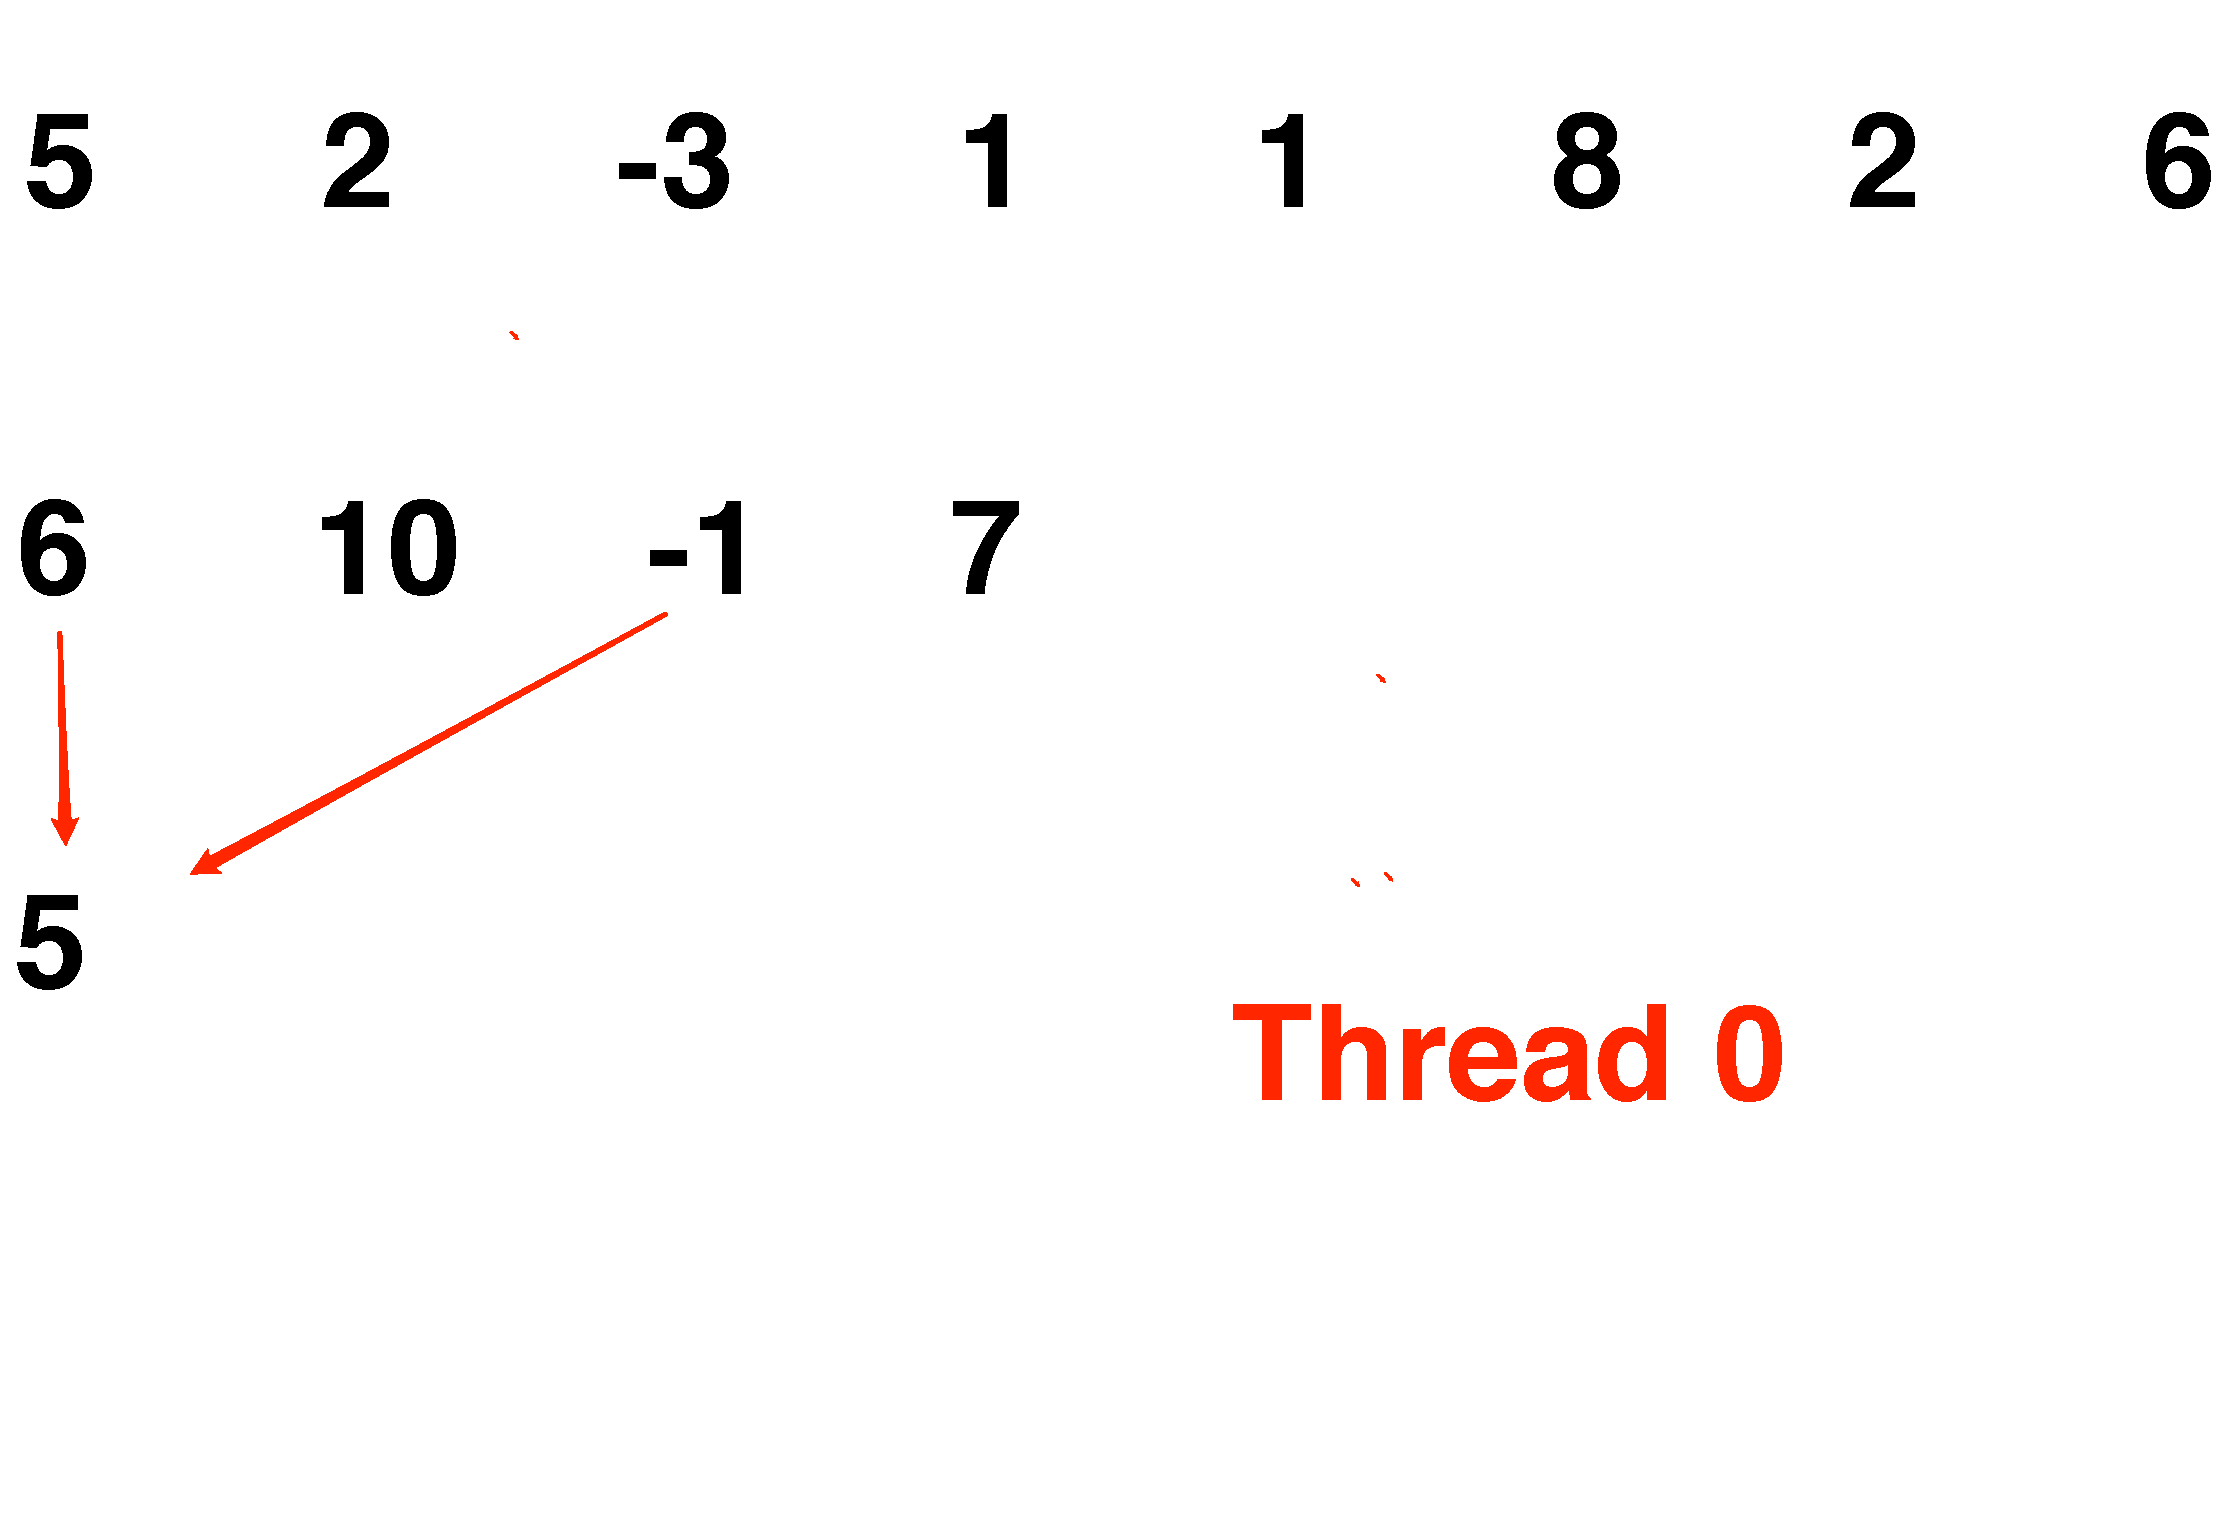
\includegraphics[scale=.25]{../../fig/psum6.pdf}
\end{frame}

\begin{frame}
\frametitle{Pairwise summation}
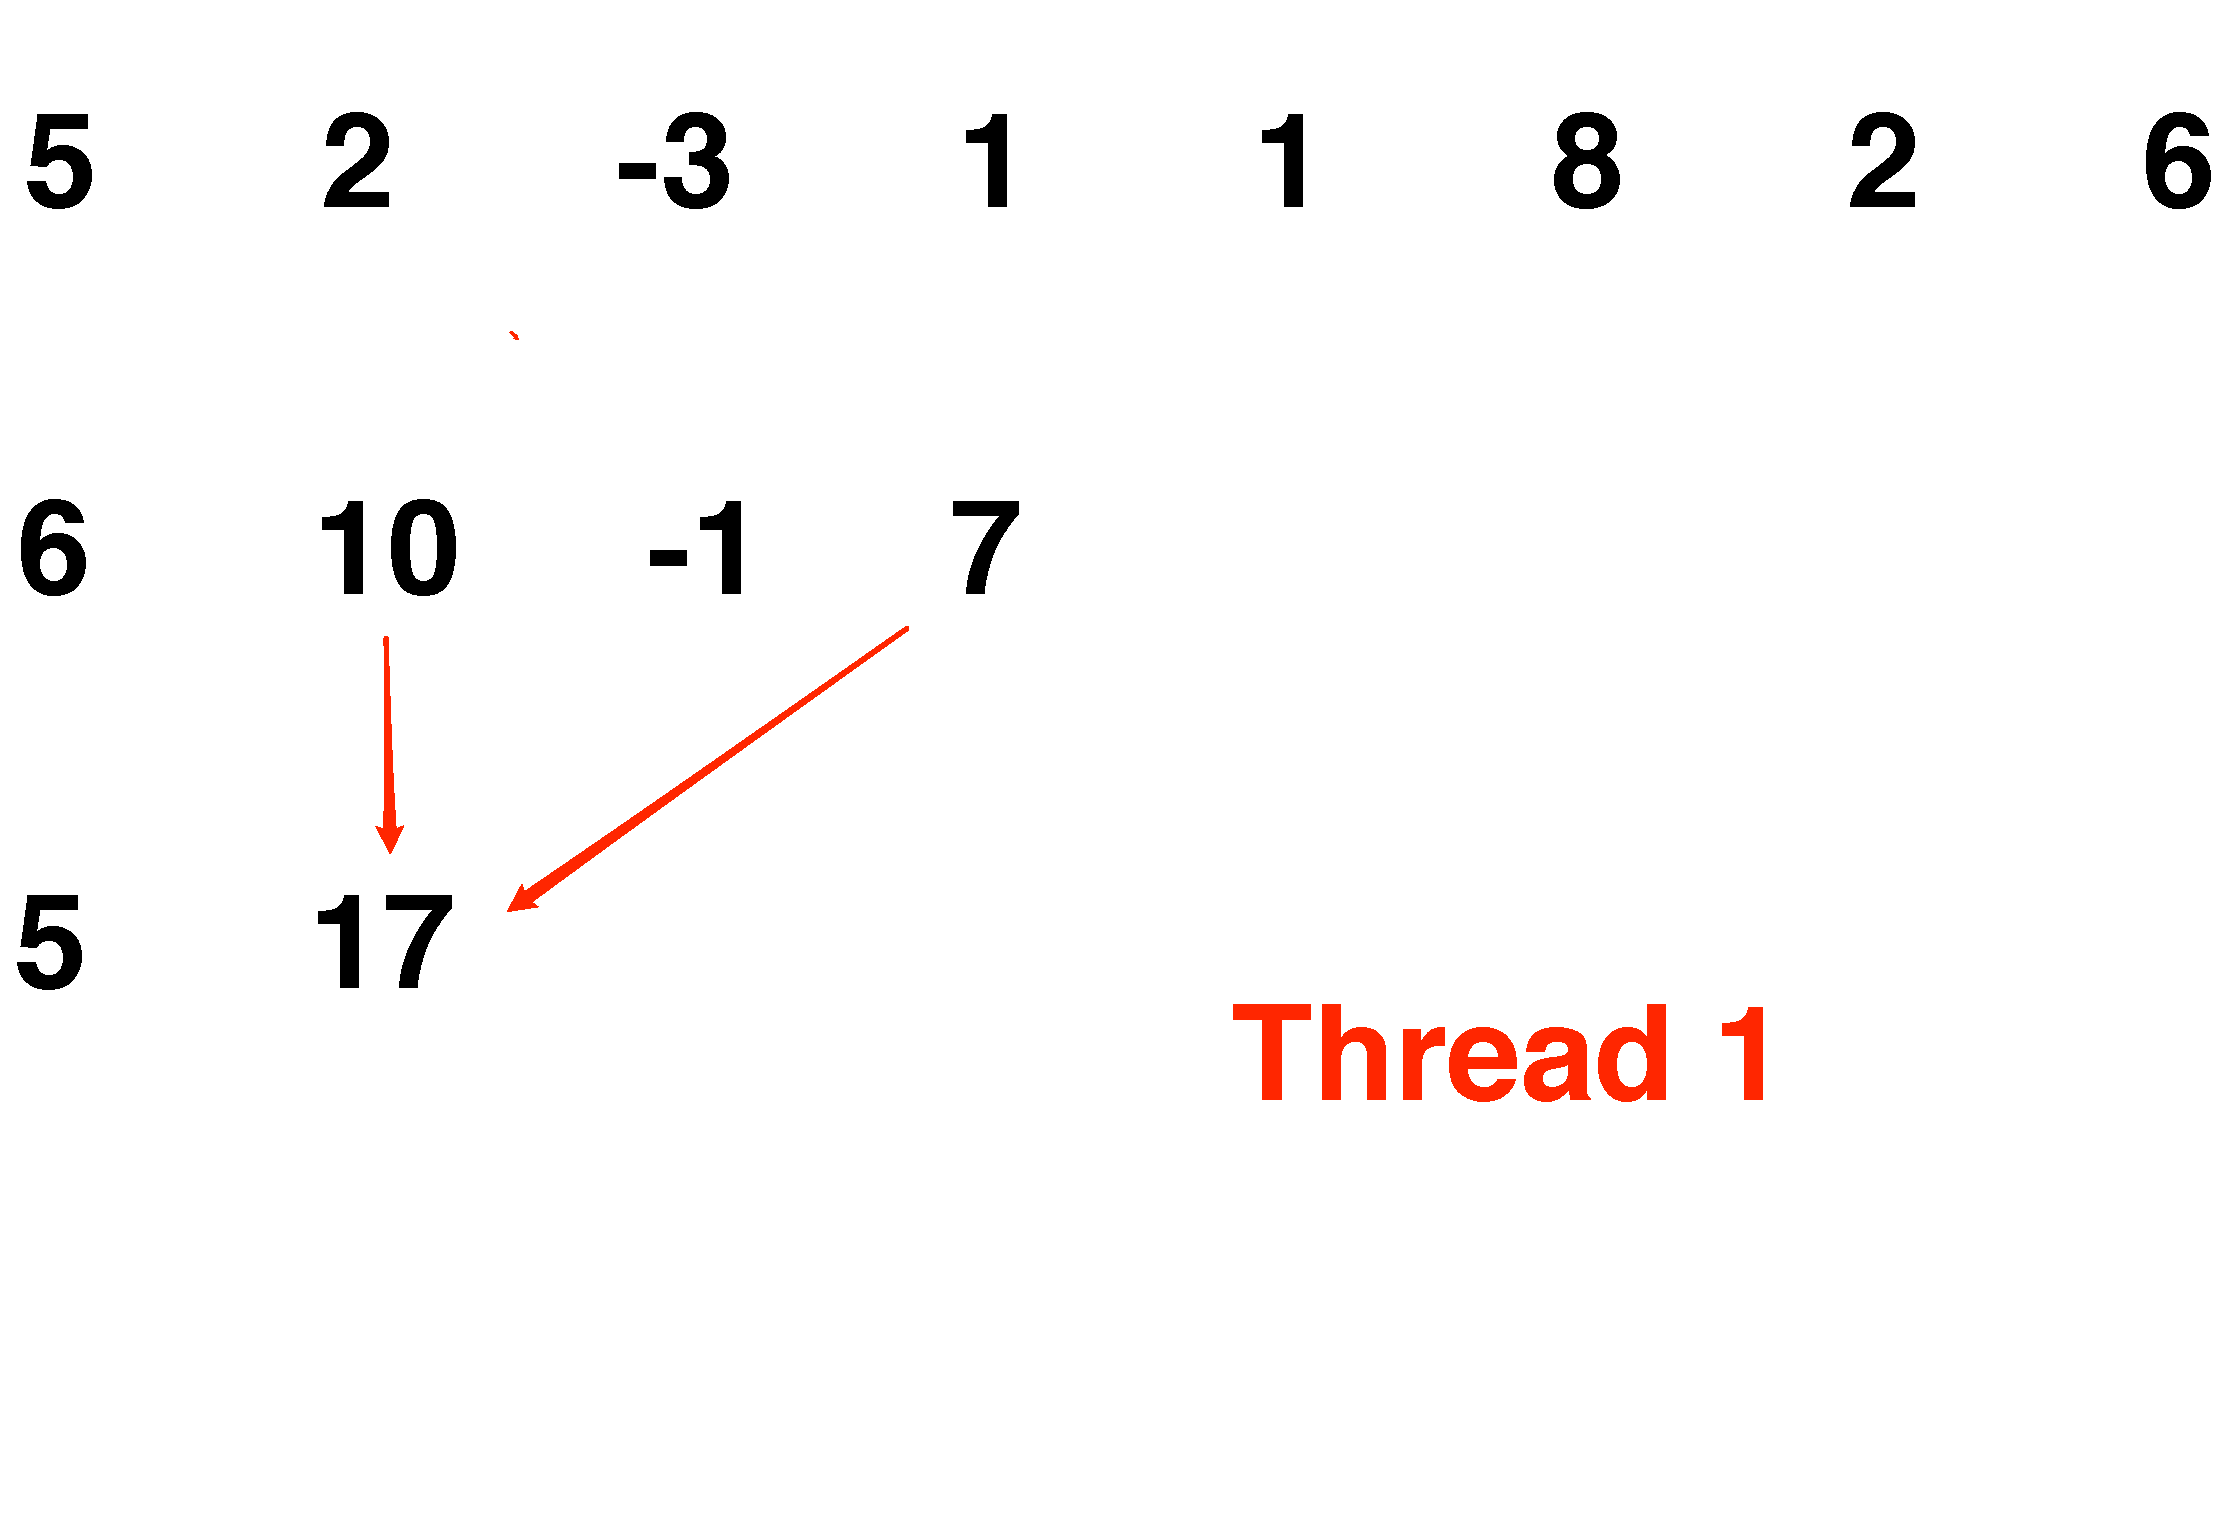
\includegraphics[scale=.25]{../../fig/psum7.pdf}
\end{frame}

\begin{frame}
\frametitle{Pairwise summation}
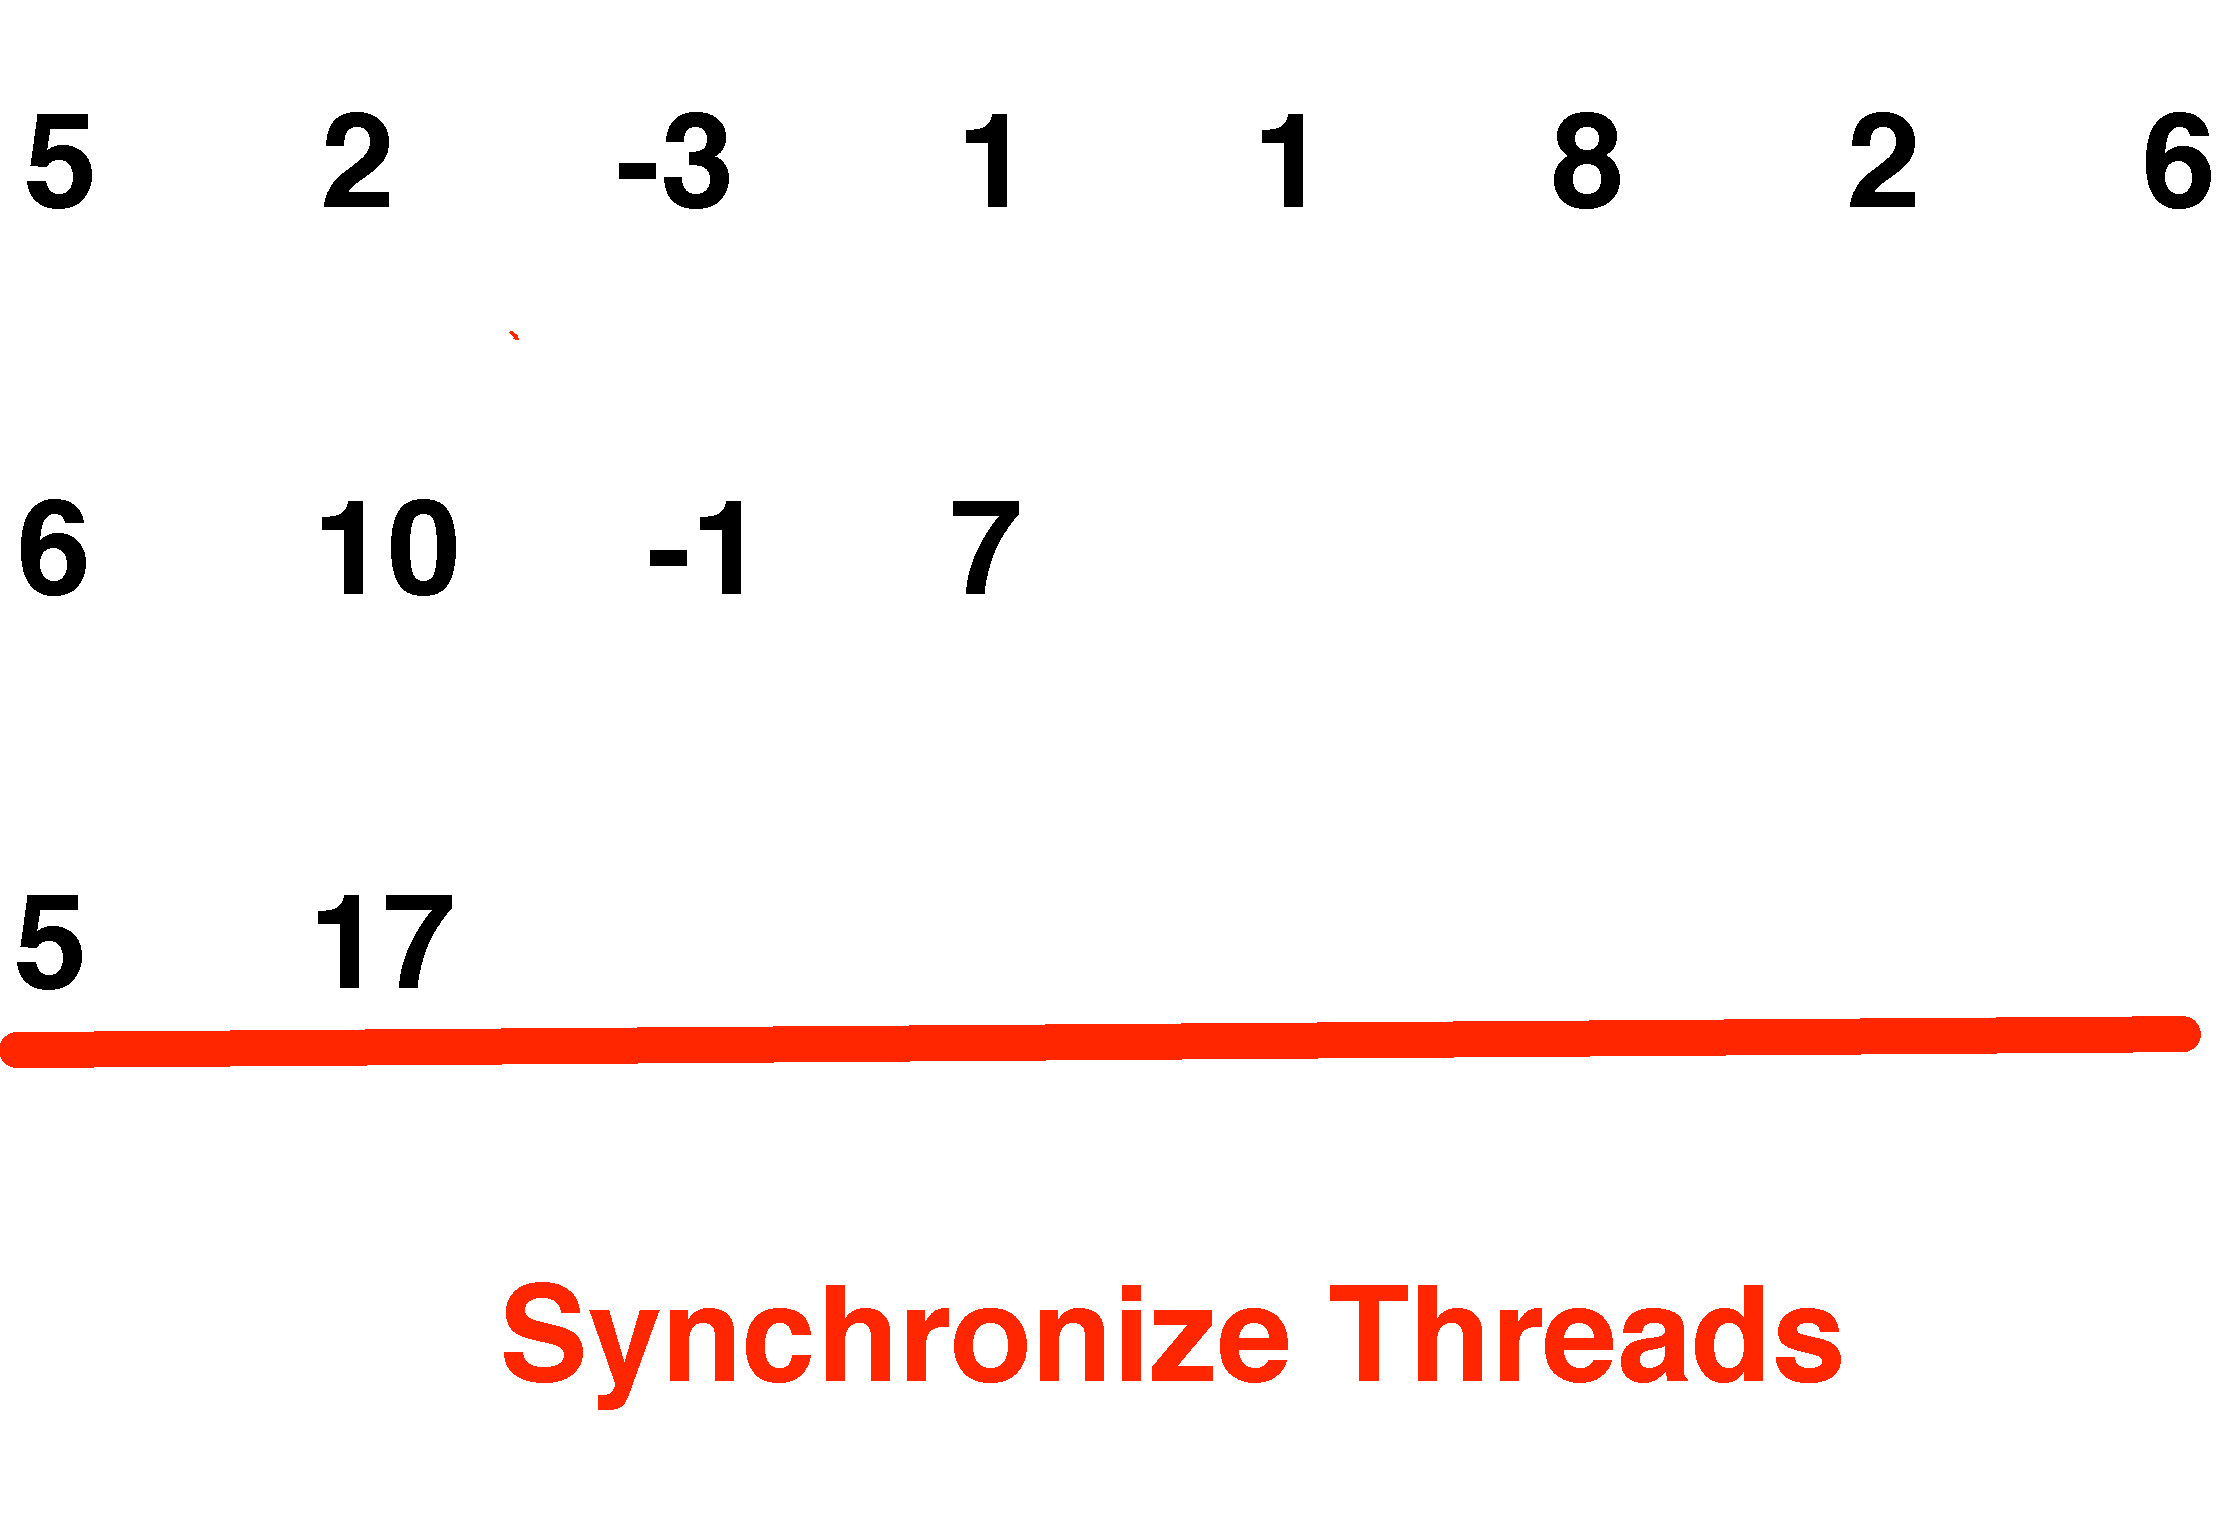
\includegraphics[scale=.25]{../../fig/psum8.pdf}
\end{frame}

\begin{frame}
\frametitle{Pairwise summation}
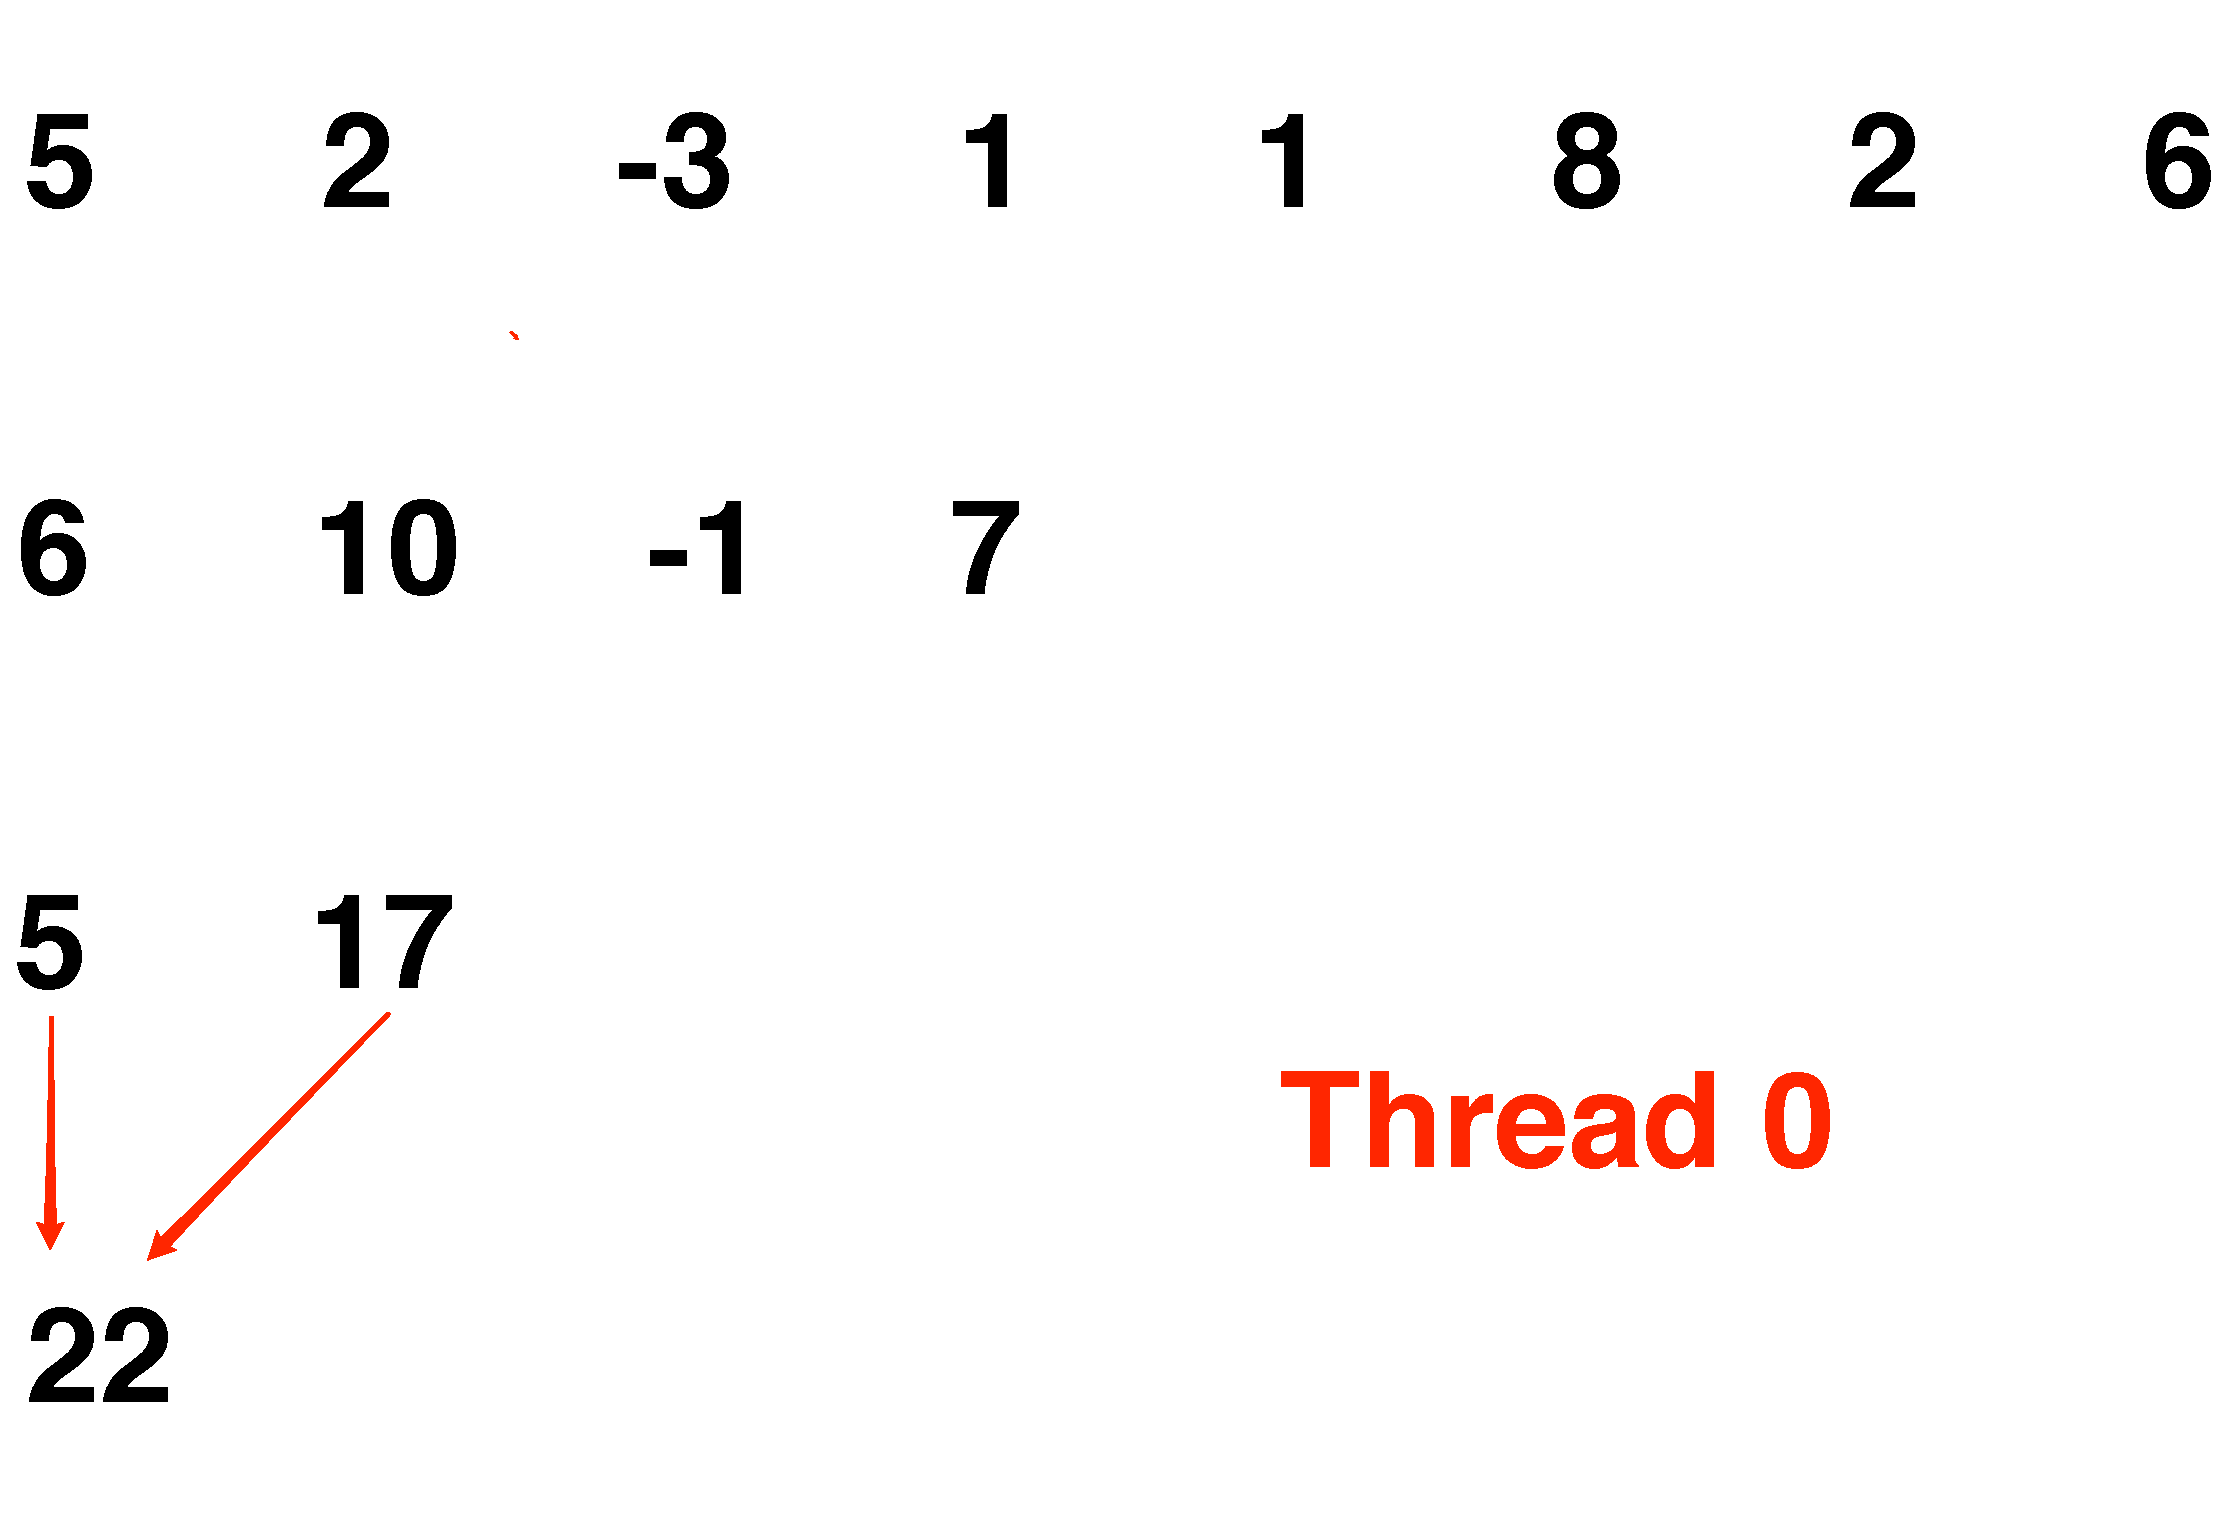
\includegraphics[scale=.25]{../../fig/psum9.pdf}
\end{frame}



\begin{frame}
\frametitle{Compare the pairwise sum to the sequential sum}
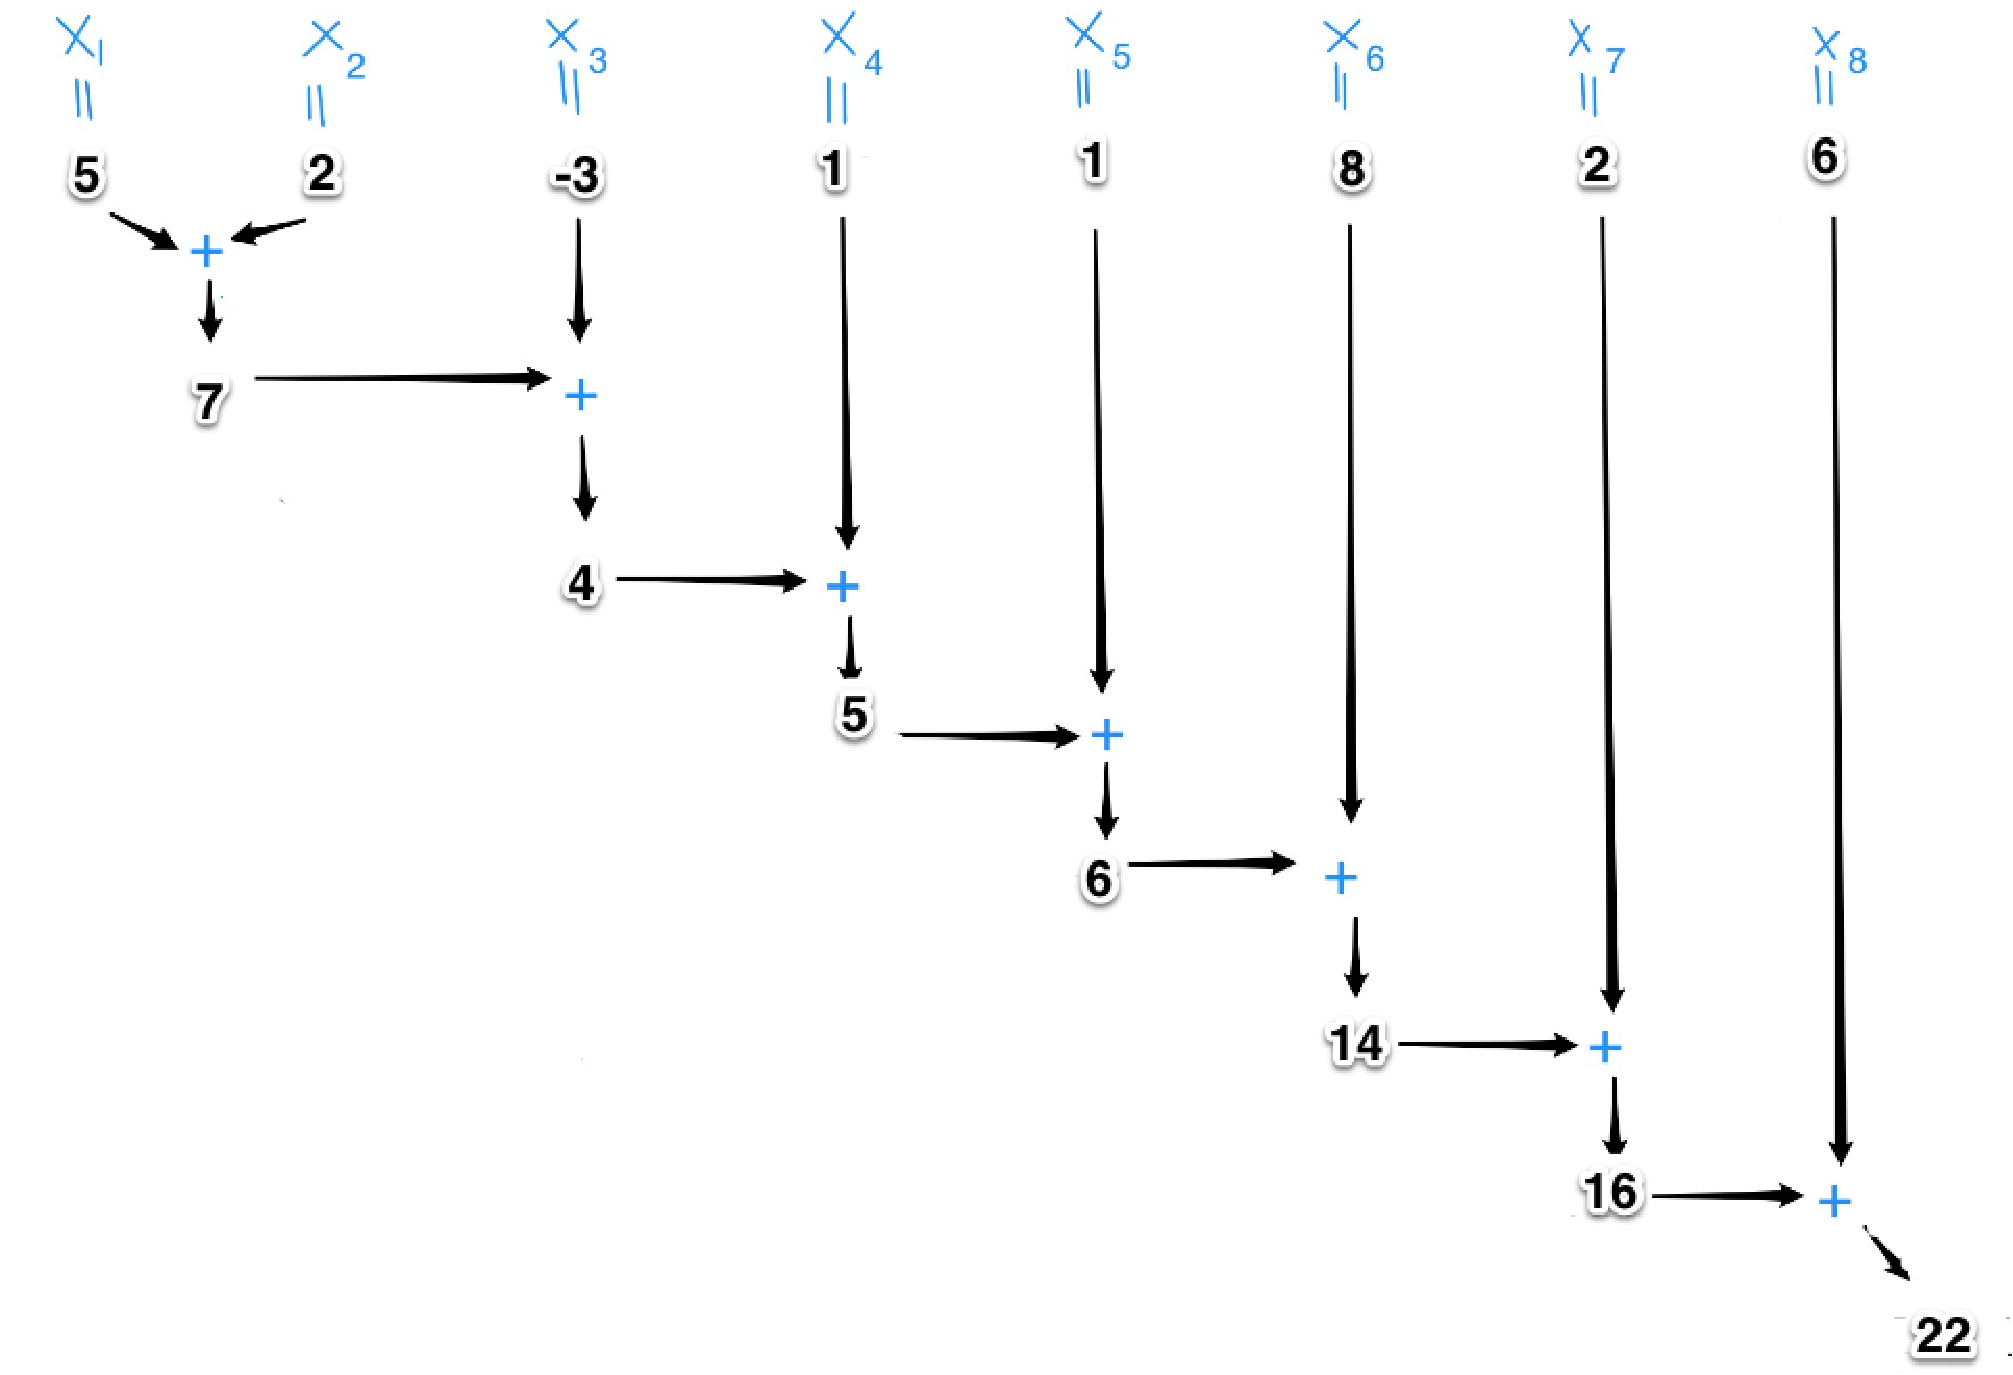
\includegraphics[scale=.25]{../../fig/sequential}
\begin{itemize}
\item The pairwise sum requires only $\log_2(n)$ sequential steps, while the sequential sum requires $n-1$ sequential steps.
\end{itemize}
\end{frame}


\begin{frame}
\frametitle{Reductions and scans}

\begin{itemize}
\item Reductions
\begin{itemize}
\pause \item Pairwise sum and pairwise multiplication are examples of reductions.
\pause \item {\bf Reduction}: an algorithm that applies some binary operation on a vector to produce a scalar.
\end{itemize}
\pause \item Scans
\begin{itemize}
\pause \item {\bf Scan (prefix sum)}: an operation on a vector that produces a sequence of partial reductions.
\pause \item Example: computing the sequence of partial sums in pairwise fashion.
\end{itemize}
\end{itemize}
\end{frame}


\subsection{Matrix multiplication}

\begin{frame}
\frametitle{Matrix multiplication} \scriptsize
\begin{itemize}\scriptsize
\item Take an $m \times n$ matrix, $A = (a_{ij})$, and an $n \times p$ matrix, $B = (b_{jk})$. Compute $C = A \cdot B$:
\begin{itemize}\scriptsize
\pause \item Write $A$ in terms of its rows: $A = \begin{bmatrix} a_{1.} \\ \vdots \\ a_{m.} \end{bmatrix}$ where $a_{i.} = \begin{bmatrix} a_{i1} & \cdots & a_{in} \end{bmatrix}$.
\pause \item Write $B$ in terms of its columns: $B = \begin{bmatrix} b_{.1} & \cdots & b_{.p} \end{bmatrix}$ where $b_{.k} = \begin{bmatrix} b_{1k}  \\ \vdots \\ b_{nk} \end{bmatrix}$
\pause \item Compute $C = A \cdot B$ by taking the product of each row of $A$ with each column of $B$:
\pause \begin{align*}
C = A \cdot B = \begin{bmatrix}
(a_{1.} \cdot b_{.1}) &  \cdots & (a_{1.} \cdot b_{.p})  \\
\vdots & \ddots & \vdots \\
(a_{m.} \cdot b_{.1})  &  \cdots & (a_{m.} \cdot b_{.p}) 
\end{bmatrix}
\end{align*}
\end{itemize}
\end{itemize}
\end{frame}


\begin{frame}
\frametitle{Parallelizing matrix multiplication}



\begin{itemize}
\item Entry $(i, k)$ of matrix $C$ is
\begin{align*}
c_{ik} &= \underbrace{a_{i1} b_{1k}} + \underbrace{a_{i2} b_{2k}} + \cdots + \underbrace{a_{in} b_{nk}} \\
&\uncover<2->{= \ c_{i1k} \ \ + \ c_{i2k} \ + \cdots + \ \ c_{ink}}
\end{align*} 

\uncover<3->{\item Assign block ($i, k$) to compute $c_{ik}$.}
\begin{enumerate}
\uncover<4->{ \item Spawn $n$ threads.}
\uncover<5->{\item Tell the $j$'th thread to compute $c_{ijk} = a_{ij} \cdot b_{jk}$. }
\uncover<6->{ \item Synchronize threads to make sure we have finished calculating $c_{i1k}, c_{i2k}, \ldots, c_{ink}$ before continuing.}
\uncover<7->{ \item Compute $c_{ik} = \sum_{j = 1}^n c_{ijk}$ as a pairwise sum.}
\end{enumerate}
\end{itemize}
\end{frame}




\begin{frame}
\frametitle{Matrix multiplication}

\begin{itemize}
\item Say I want to compute $A \cdot B$, where: 
\end{itemize}

\pause \begin{align*}
A = \begin{bmatrix} 1 & 2 \\
-1 & 5 \\
7 & -9 \end{bmatrix} \quad 
B = \begin{bmatrix}
8 & 8 & 7 \\
3 & 5 & 2
\end{bmatrix}
\end{align*}


\pause \begin{itemize}
\item I write the multiplication as an array of products: 
\end{itemize}

\pause \begin{align*}\scriptsize
C =  \begin{bmatrix}
\left ( \begin{bmatrix} 1 & 2\end{bmatrix} \cdot \begin{bmatrix} 8 \\ 3\end{bmatrix}  \right ) & \left (  \begin{bmatrix} 1 & 2 \end{bmatrix} \cdot \begin{bmatrix} 8 \\ 5 \end{bmatrix}  \right ) & \left ( \begin{bmatrix} 1 & 2 \end{bmatrix} \cdot \begin{bmatrix} 7 \\ 2\end{bmatrix} \right ) \\ \\
\left ( \begin{bmatrix} -1 & 5\end{bmatrix} \cdot \begin{bmatrix} 8 \\ 3 \end{bmatrix}  \right) & \left (  \begin{bmatrix} -1 & 5 \end{bmatrix} \cdot \begin{bmatrix} 8 \\ 5 \end{bmatrix} \right ) & \left (\begin{bmatrix} -1 & 5 \end{bmatrix} \cdot \begin{bmatrix} 7 \\ 2\end{bmatrix} \right )\\ \\
\left ( \begin{bmatrix} 7 & -9 \end{bmatrix} \cdot \begin{bmatrix} 8 \\ 3 \end{bmatrix}  \right) & \left (  \begin{bmatrix}  7 & -9\end{bmatrix} \cdot \begin{bmatrix} 8 \\ 5 \end{bmatrix} \right ) & \left (\begin{bmatrix} 7 & -9 \end{bmatrix} \cdot \begin{bmatrix} 7 \\ 2\end{bmatrix} \right )\\
\end{bmatrix}
\end{align*}
\end{frame}

\begin{frame}
\frametitle{Matrix multiplication}
\begin{itemize}
\item We don't need to synchronize blocks because they operate independently.
\end{itemize}
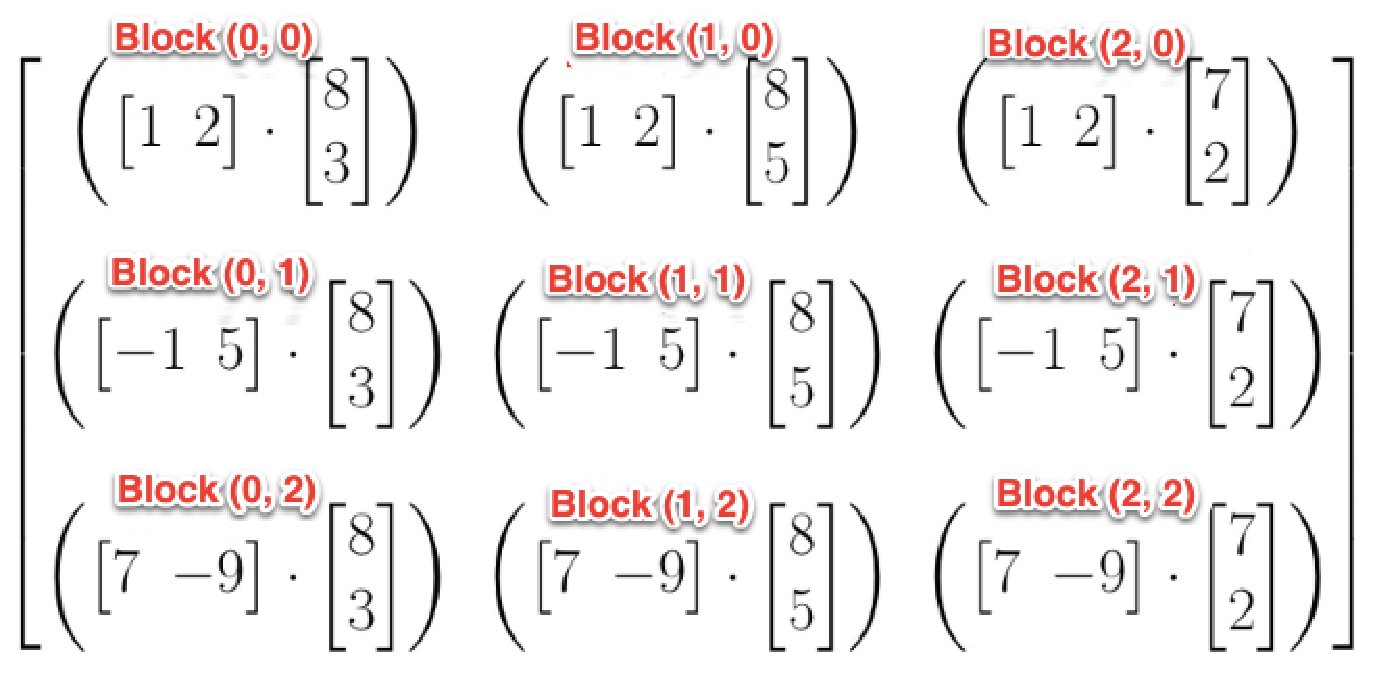
\includegraphics[scale=0.4]{../../fig/mat}
\end{frame}

\begin{frame}
\frametitle{Matrix multiplication}
\begin{itemize}
\item Consider block (0, 0), which computes $\begin{bmatrix} 1 & 2 \end{bmatrix} \cdot \begin{bmatrix} 8 \\ 3 \end{bmatrix}$
\end{itemize}
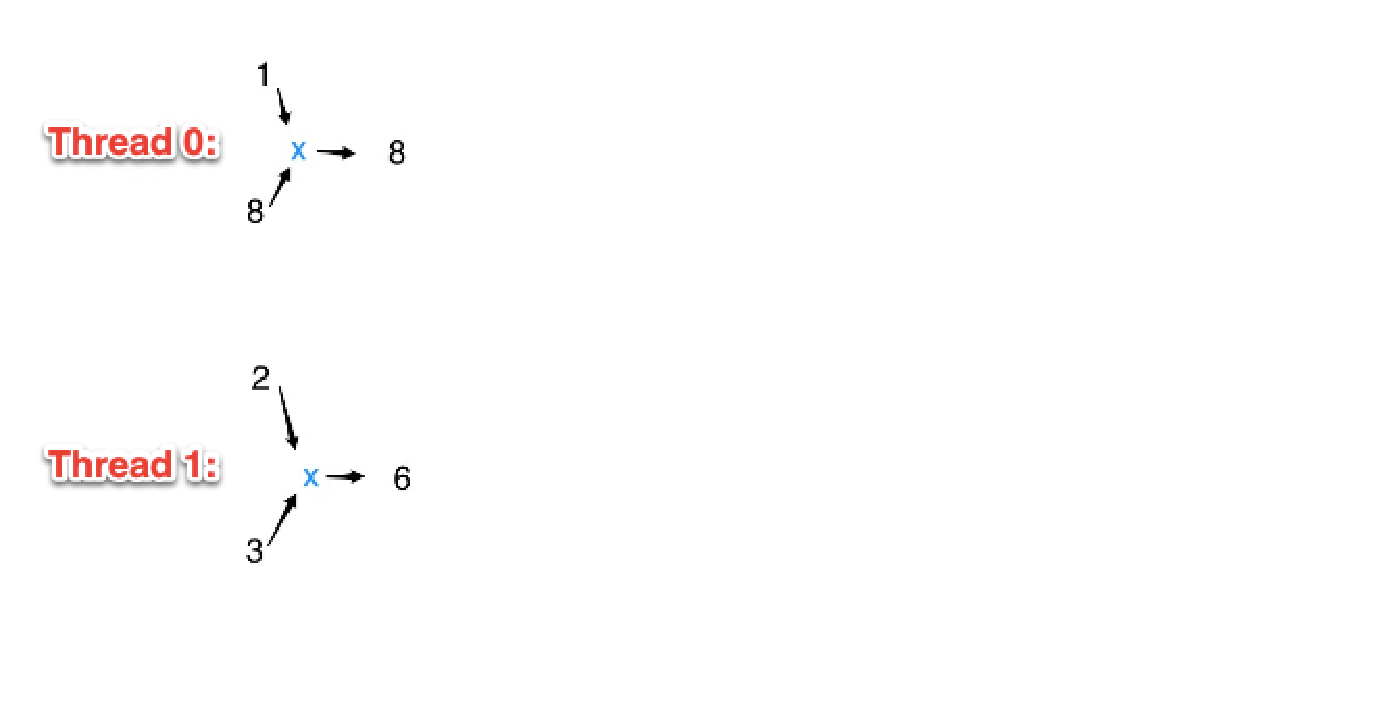
\includegraphics[scale=0.4]{../../fig/matb1}
\end{frame}

\begin{frame}
\frametitle{Matrix multiplication}
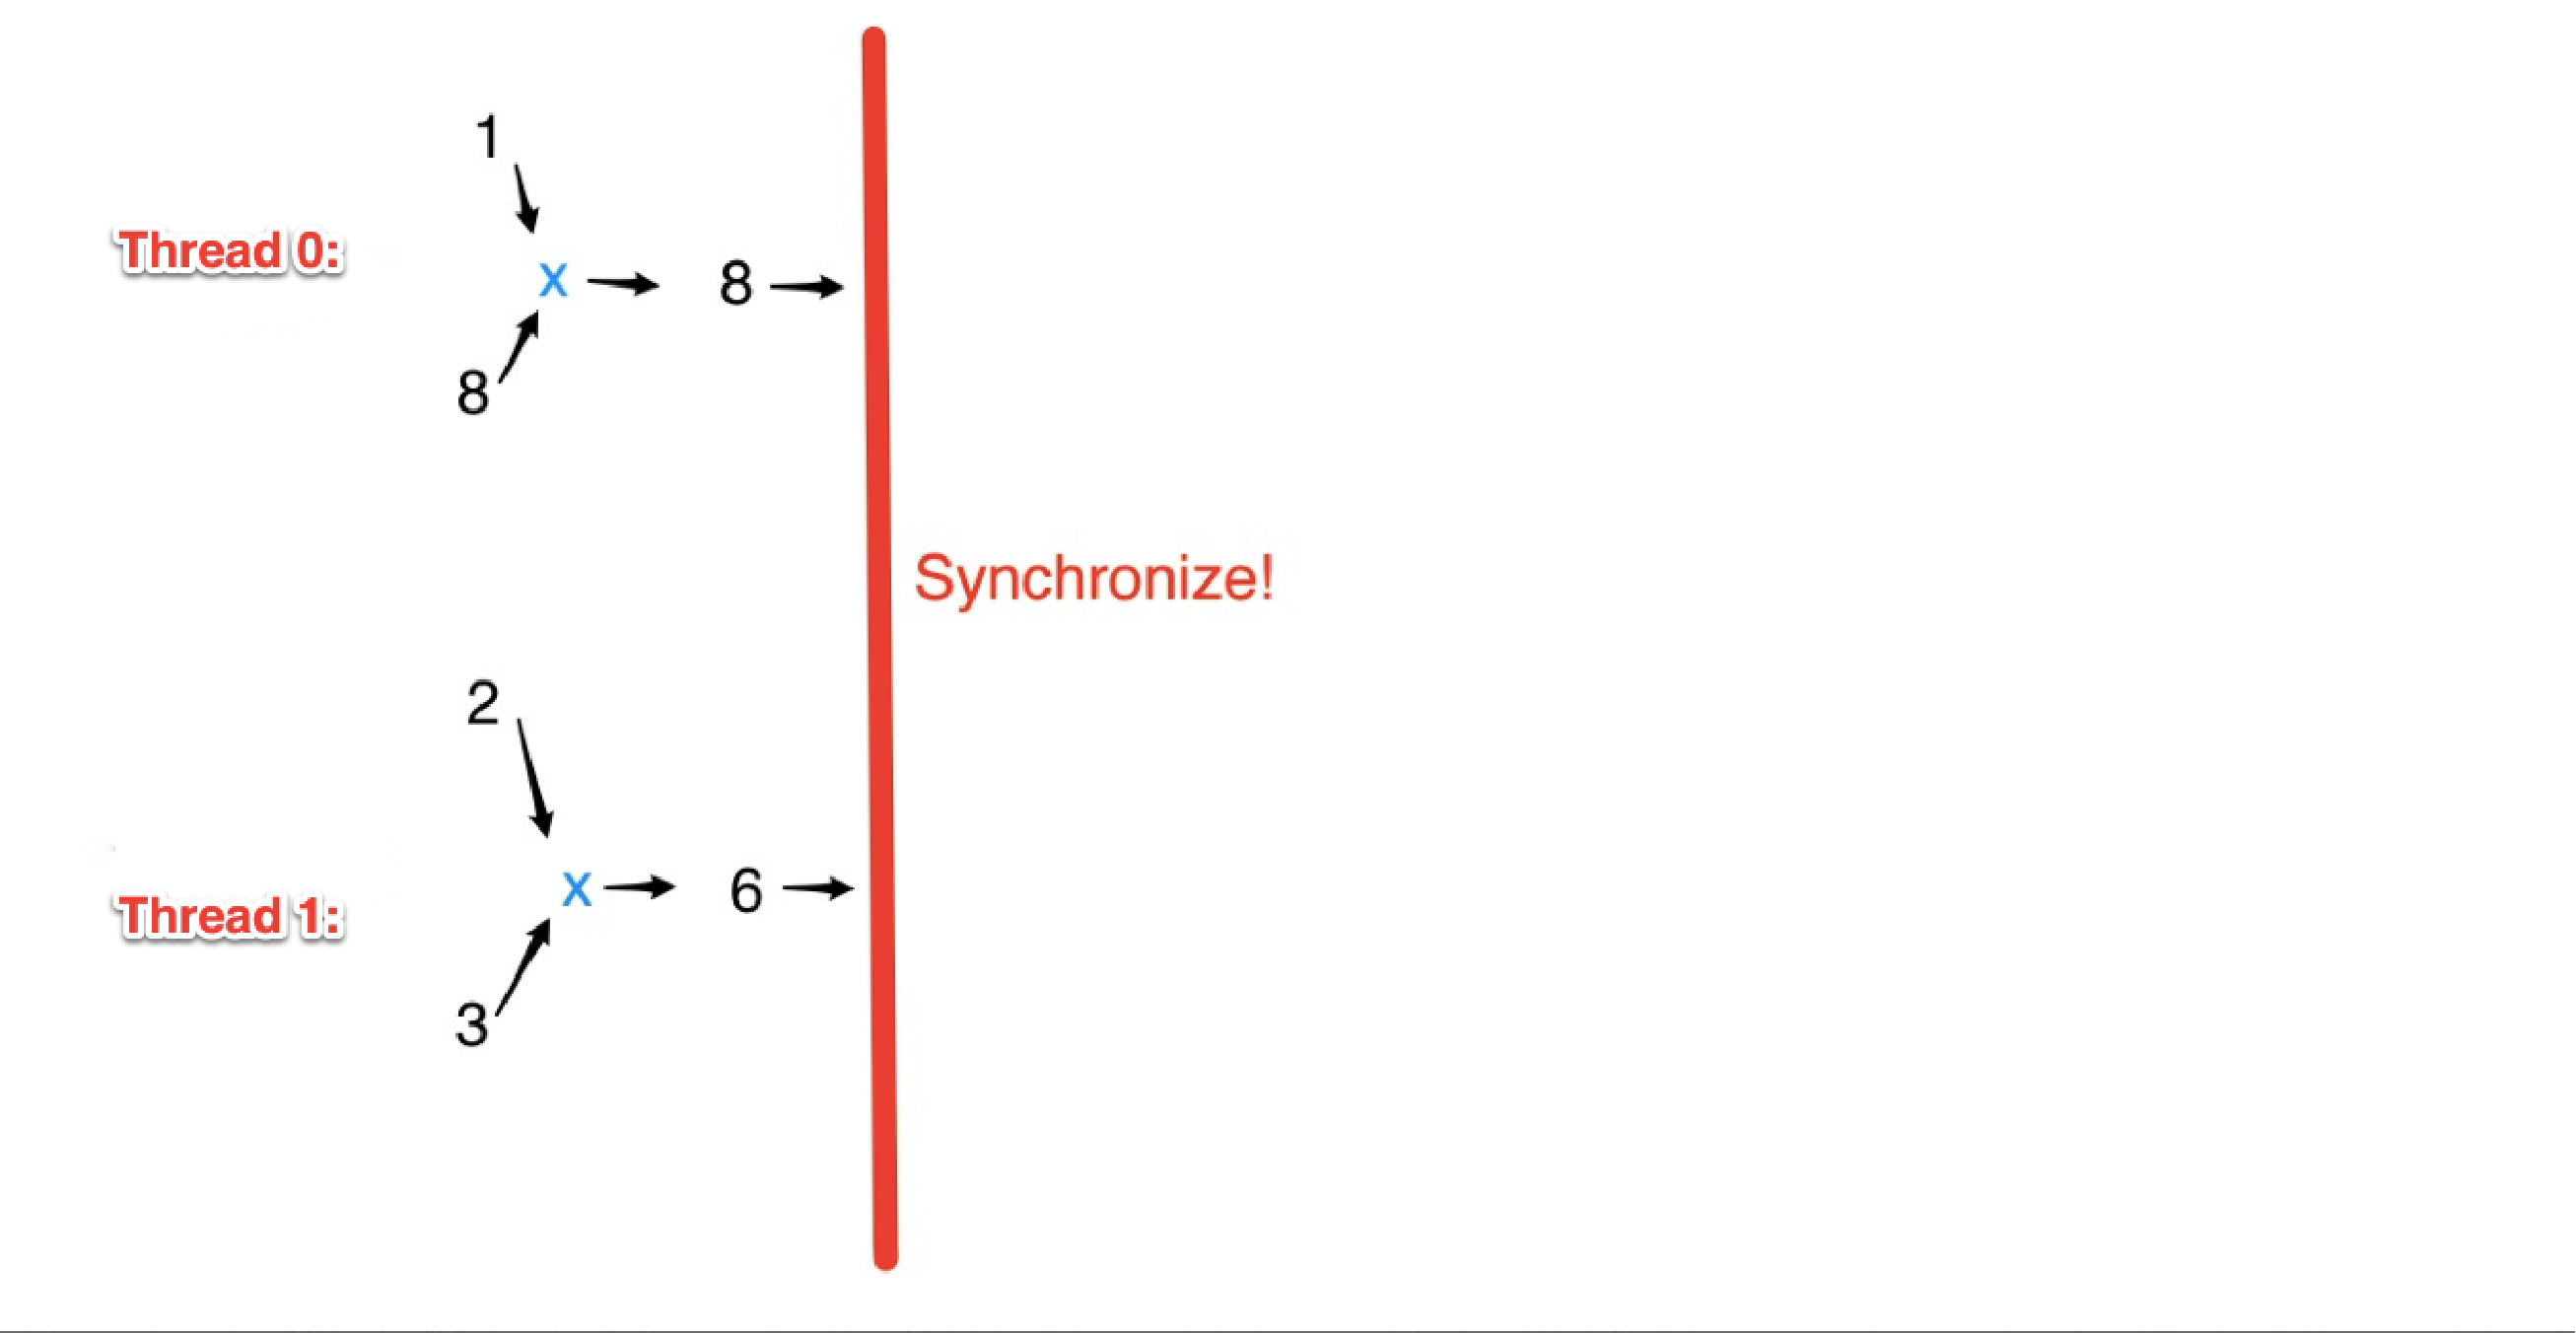
\includegraphics[scale=0.2]{../../fig/matb2}
\end{frame}

\begin{frame}
\frametitle{Matrix multiplication}
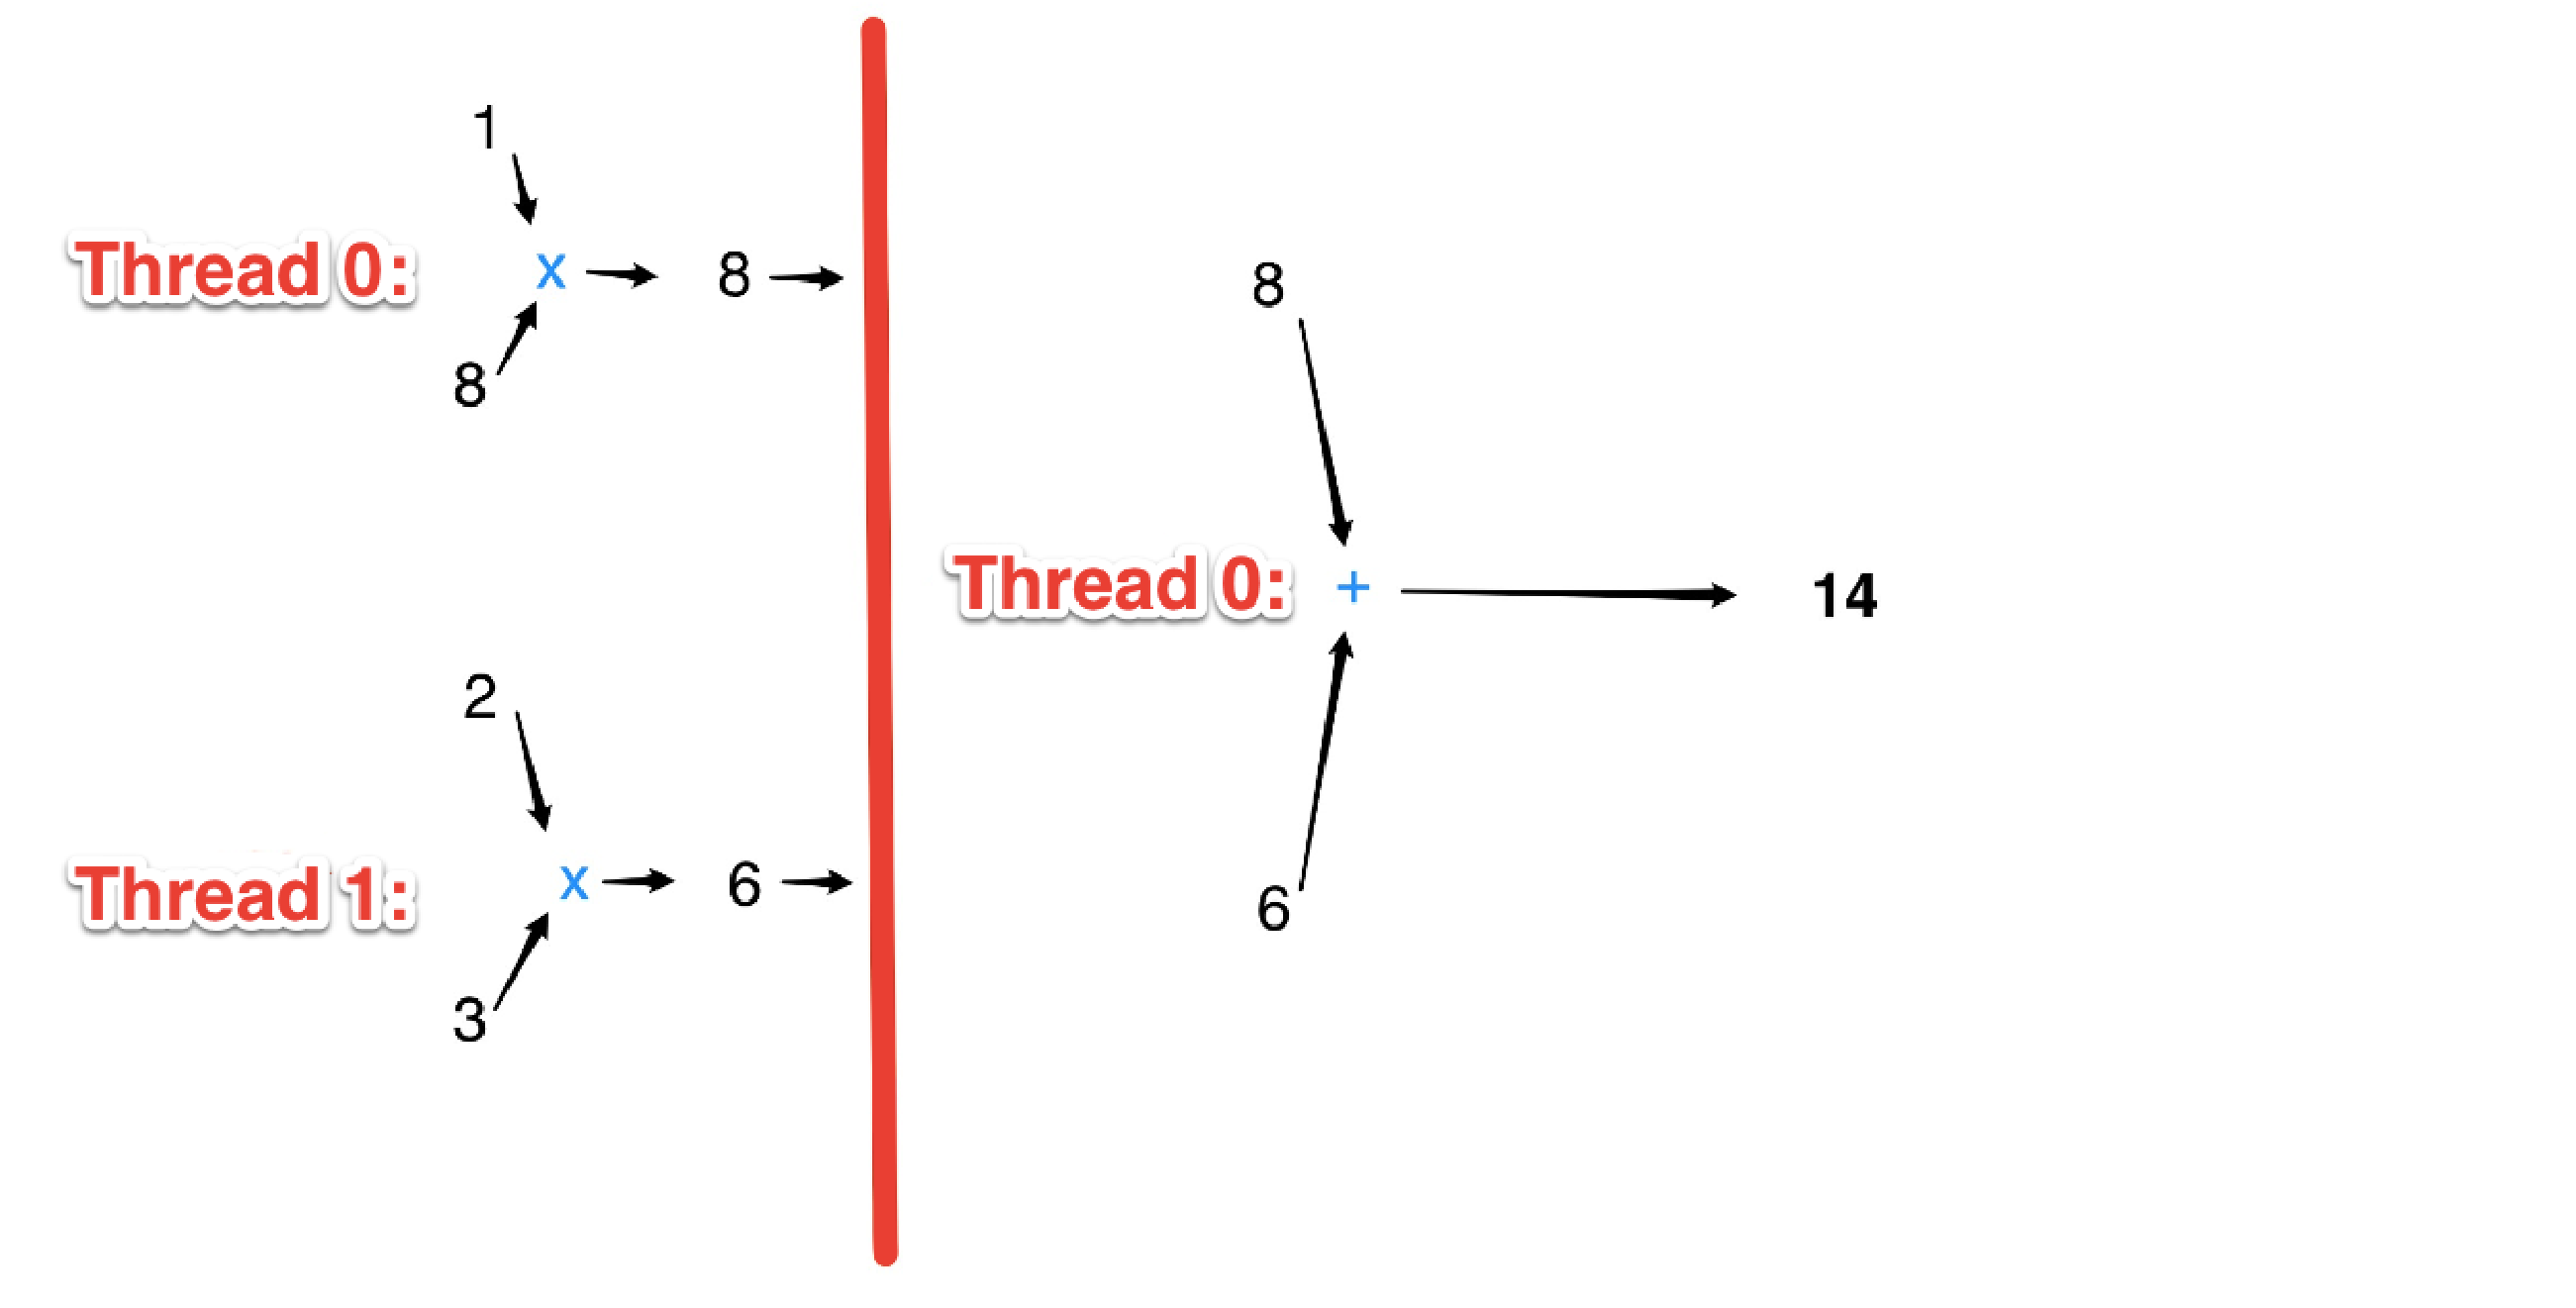
\includegraphics[scale=0.2]{../../fig/matb3}
\end{frame}



\subsection{K-means clustering}

\begin{frame}
\frametitle{Lloyd's K-means algorithm}
\begin{itemize}
\item Cluster $N$ vectors in Euclidian space into $K$ groups. 
\end{itemize}

\begin{center}
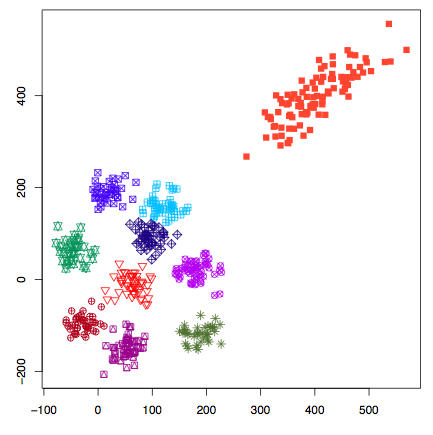
\includegraphics[scale=.4]{../../fig/kmeans0.png}
\end{center}
\end{frame}

\begin{frame}
\frametitle{Step 1: choose initial cluster centers.}
\begin{center}
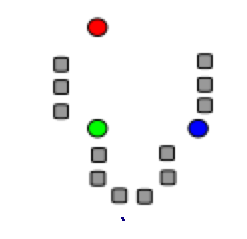
\includegraphics[scale=.6]{../../fig/kmeans1.png}
\end{center}
\begin{itemize}
\item The circles are the cluster means, the squares are the data points, and the color indicates the cluster.
\end{itemize}
\end{frame}

\begin{frame}
\frametitle{Step 2: assign each data point (square) to its closest center (circle).}
\begin{center}
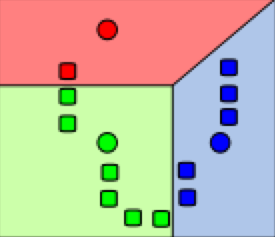
\includegraphics[scale=.6]{../../fig/kmeans2.png}
\end{center}
\end{frame}

\begin{frame}
\frametitle{Step 3: update the cluster centers to be the within-cluster data means.}
\begin{center}
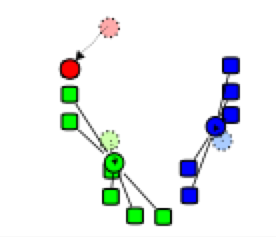
\includegraphics[scale=.6]{../../fig/kmeans3.png}
\end{center}
\end{frame}

\begin{frame}
\frametitle{Repeat step 2: reassign points to their closest cluster centers.}
\begin{center}
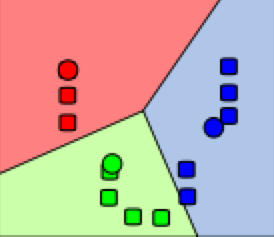
\includegraphics[scale=.6]{../../fig/kmeans4.png}
\end{center}
\begin{itemize}
\item $\ldots$ and repeat until convergence.
\end{itemize}
\end{frame}

\begin{frame}
\frametitle{Parallel K-means}
\begin{itemize}
\item Step 2: assign points to closest cluster centers.
\begin{itemize}
\pause \item Spawn $N$ blocks with $K$ threads each.
\pause \item Let thread $(n, k)$ compute the distance between data point $n$ and cluster center $k$.
\pause \item Synchronize threads.
\pause \item Let thread $(n, 1)$ assign data point $n$ to its nearest cluster center.
\end{itemize}
\pause \item Step 3: recompute cluster centers.
\begin{itemize}
\pause \item Spawn one block for each cluster.
\pause \item Within each block, compute the mean of the data in the corresponding cluster.
\end{itemize}
\end{itemize}
\end{frame}



\subsection{Markov chain Monte Carlo}

\begin{frame}
\frametitle{Markov chain Monte Carlo}
\begin{itemize}
\item Consider a bladder cancer data set:
\begin{itemize}  \scriptsize
\pause \item Available from http://ratecalc.cancer.gov/.
\pause \item Rates of death from bladder cancer of white males from 2000 to 2004 in each county in the USA.
\end{itemize}
\pause \item Let:
\begin{itemize}  \scriptsize
\item $y_k$ = number of observed deaths in county $k$.
\pause \item $n_k$ = the number of person-years in county $k$ divided by 100,000.
\pause \item $\theta_k$ = expected number of deaths per 100,000 person-years.
\end{itemize} 
\pause \item The model:
\begin{align*}
\uncover<7->{y_k} &\uncover<7->{\stackrel{\text{ind}}{\sim} \text{Poisson}(n_k \cdot \theta_k)}\\
\uncover<8->{\theta_k} &\uncover<8->{\stackrel{\text{iid}}{\sim} \text{Gamma}(\alpha, \ \beta)}\\
\uncover<9->{\alpha} & \uncover<9->{\sim \text{Uniform}(0, a_0)} \\
\uncover<10->{\beta} & \uncover<10->{\sim \text{Uniform}(0, b_0)}
\end{align*}
\uncover<11->{\begin{itemize}
\item Also assume $\alpha$ and $\beta$ are independent and fix $a_0$ and $b_0$.
\end{itemize}}
\end{itemize}
\end{frame}

\begin{frame}
\frametitle{Full conditional distributions} \scriptsize
\begin{itemize}
\item We want to sample from the joint posterior,
\end{itemize}

\begin{align*}
p(\vc{\theta}, \alpha, \beta \mid \vc{y}) &\propto p(\vc{y} \mid \vc{\theta}, \alpha, \beta) p(\vc{\theta}, \alpha, \beta) \\
&\uncover<2->{\propto p(\vc{y} \mid \vc{\theta}, \alpha, \beta) p(\vc{\theta} \mid \alpha, \beta) p(\alpha, \beta)} \\
&\uncover<3->{\propto p(\vc{y} \mid \vc{\theta}, \alpha, \beta) p(\vc{\theta} \mid \alpha, \beta) p(\alpha)p(\beta)} \\
&\uncover<4->{\propto \prod_{k = 1}^K [p(y_k \mid \theta_k, n_k) p(\theta_k \mid \alpha, \beta)] p(\alpha) p(\beta)} \\
&\uncover<5->{\propto \prod_{k = 1}^K \left [e^{-n_k \theta_k} \theta_k^{y_k} \frac{\beta^\alpha}{\Gamma(\alpha)} \theta_k^{\alpha - 1} e^{-\theta_k \beta}\right ] I(0 < \alpha < a_0) I(0 < \beta < b_0) }
\end{align*}
\begin{itemize}
\uncover<6->{\item We iteratively sample from the full conditional distributions.}
\end{itemize}
\begin{align*}
\uncover<7->{\alpha} &\uncover<7->{\leftarrow p(\alpha \mid \vc{y}, \vc{\theta}, \beta)}  \\
\uncover<8->{\beta} &\uncover<8->{\leftarrow p(\beta \mid \vc{y}, \vc{\theta}, \alpha)} \\
\uncover<9->{\theta_k} &\uncover<9->{\leftarrow p(\theta_k \mid \vc{y}, \vc{\theta}_{-k}, \alpha, \beta) \qquad \Leftarrow \text{IN PARALLEL!}} 
\end{align*}


\end{frame}



\begin{frame}
\frametitle{Full conditional distributions}

\begin{align*}
\uncover<2->{p(\theta_k \mid \vc{y}, \vc{\theta_{-k}}, \alpha, \beta)} & \uncover<2->{\propto p(\vc{\theta}, \alpha, \beta \mid \vc{y})} \\
&\uncover<3->{\propto e^{-n_k \theta_k} \theta_k^{y_k} \theta_k^{\alpha - 1} e^{- \theta_k} \beta} \\
&\uncover<4->{= \theta_k^{y_k + \alpha - 1} e^{-\theta_k(n_k + \beta)}} \\
&\uncover<5->{\propto \text{Gamma}(y_k + \alpha, \ n_k + \beta)}
\end{align*}




\end{frame}

\begin{frame} 
\frametitle{Conditional distributions of $\alpha$ and $\beta$} \small
\begin{align*}
p(\alpha \mid \vc{y}, \vc{\theta}, \beta) &\propto p(\vc{\theta}, \alpha, \beta \mid \vc{y}) \\
&\uncover<2->{\propto \prod_{k = 1}^K \left [ \theta_k^{\alpha - 1} \frac{\beta^\alpha}{\Gamma(\alpha)} \right ] I(0 < \alpha < a_0)} \\
&\uncover<3->{=\left (\prod_{k = 1}^K \theta_k \right )^\alpha \beta^{K \alpha} \Gamma(\alpha)^{-K} I(0 < \alpha < a_0)} \\ \\
\uncover<4->{p(\beta \mid \vc{y}, \vc{\theta}, \alpha)} &\uncover<4->{\propto p(\vc{\theta}, \alpha, \beta \mid \vc{y})} \\
&\uncover<5->{\propto \prod_{k = 1}^K \left [ e^{-\theta_k \beta} \beta^\alpha \right ] I(0 < \beta < b_0)} \\
&\uncover<6->{=\beta^{K \alpha} e^{- \beta \sum_{k = 1}^K \theta_k} I(0 < \beta < b_0)} \\
&\uncover<7->{\propto \text{Gamma}\left (K \alpha + 1, \ \sum_{k = 1}^K \theta_k \right) I(0 < \beta < b_0)}
\end{align*}
\end{frame}



\begin{frame}
\frametitle{Summarizing the Gibbs sampler}
\begin{enumerate}
\item Sample $\vc{\theta}$ from from its full conditional.
\begin{itemize}
\pause \item Draw the $\theta_k$'s \emph{in parallel} from independent Gamma($y_k + \alpha$, $n_k + \beta$) distributions.
\pause \item In other words, assign each thread to draw an individual $\theta_k$ from its Gamma($y_k + \alpha$, $n_k + \beta$) distribution.
\end{itemize}
\pause \item Sample $\alpha$ from its full conditional using a random walk Metropolis step.
\pause \item Sample $\beta$ from its full conditional (truncated Gamma) using the inverse cdf method if $b_0$ is low or a non-truncated Gamma if $b_0$ is high.
\end{enumerate}

\end{frame}











\begin{frame}[fragile]
\frametitle{Preview: a bare bones CUDA C workflow}
\begin{lstlisting}
#include <stdio.h> 
#include <stdlib.h> 
#include <cuda.h>
#include <cuda_runtime.h> 

__global__ void some_kernel(...){...}

int main (void){ 
  // Declare all variables.
  ...
  // Allocate host memory.
  ...
  // Dynamically allocate device memory for GPU results.
  ...
  // Write to host memory.
  ... 
  // Copy host memory to device memory.
  ...
\end{lstlisting}
\end{frame}



\begin{frame}[fragile]
\frametitle{Preview: a bare bones CUDA C workflow}
\begin{lstlisting}
  // Execute kernel on the device.
  some_kernel<<< num_blocks, num_theads_per_block >>>(...);
  
  // Write GPU results in device memory back to host memory.
  ...
  // Free dynamically-allocated host memory
  ...
  // Free dynamically-allocated device memory    
  ...
}
\end{lstlisting}
\end{frame}

\begin{frame}
\frametitle{Outline}
\tableofcontents
\end{frame}

\begin{frame}
\frametitle{Resources}
\begin{enumerate}[1. ]
\item J. Sanders and E. Kandrot. \emph{CUDA by Example.} Addison-Wesley, 2010.
\pause \item Prof. Jarad Niemi's STAT 544 lecture notes.
\end{enumerate}
\end{frame}

\begin{frame}
\frametitle{That's all for today.}
\begin{itemize}
\item Series materials are available at \url{http://will-landau.com/gpu}.
\end{itemize}
\end{frame}


\end{document}